\chapter{Theoretical introduction}

\section{Superconducting microwave coplanar waveguide resonators}

\subsection{Equations for quality factors}

The total quality factor of a microwave transmission line resonator (TLR) $Q_l$ (loaded quality factor) can be calculated as a sum of two parts -- the internal and external quality factors. The internal quality factor $Q_i$ describes how excitations leave the resonator in the absence of coupling to any external circuitry, so damping in this case comes from the internal defects (i.e., resonant two-level systems) in the resonator itself. When, however, the resonator is coupled to the external circuitry having some active resistance, the damping is enhanced and the total Q-factor is reduced according to the following expression:
\begin{equation}
Q_l^{-1} = Q_i^{-1}+Q_e^{-1},
\label{eq:qfactor}
\end{equation}
where $Q_e$ is determined by the value of the externally connected resistance and the way of its connection.

\begin{figure}
\captionsetup[subfigure]{width = 0.9\textwidth, justification=normal}
\centering
\begin{subfigure}[t]{0.48\textwidth}
\centering
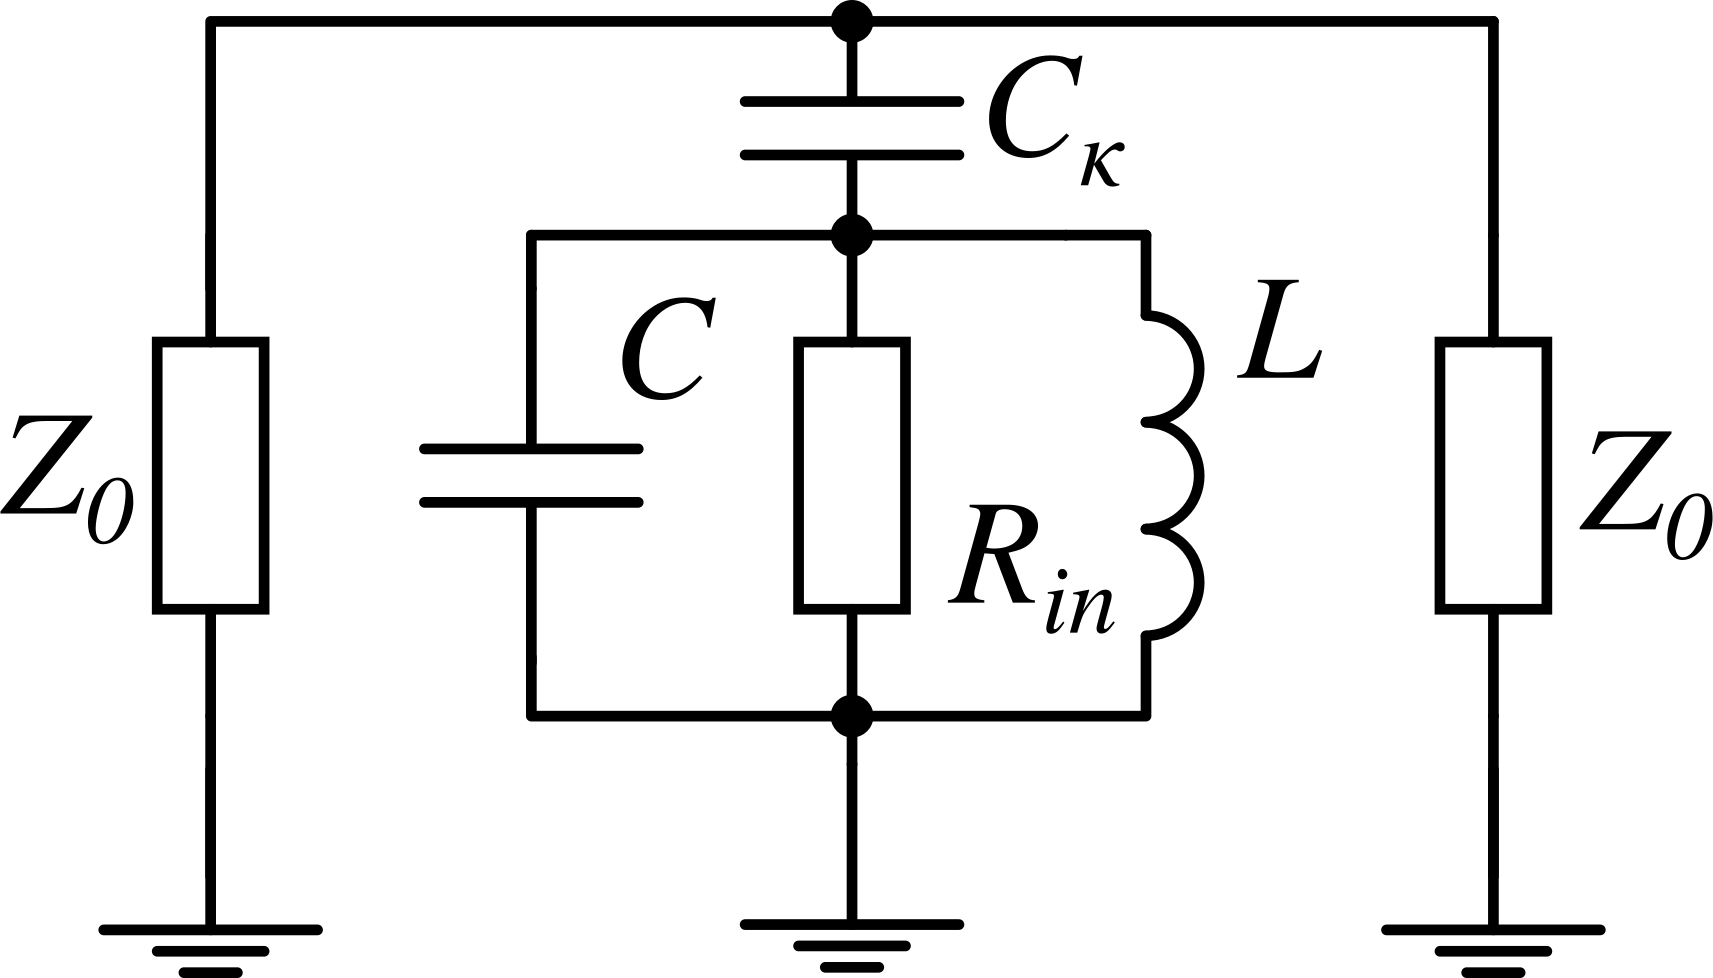
\includegraphics[width=0.9\textwidth]{resonator}
\caption{Real world circuit configuration.}
\end{subfigure}
\begin{subfigure}[t]{0.48\textwidth}
\centering
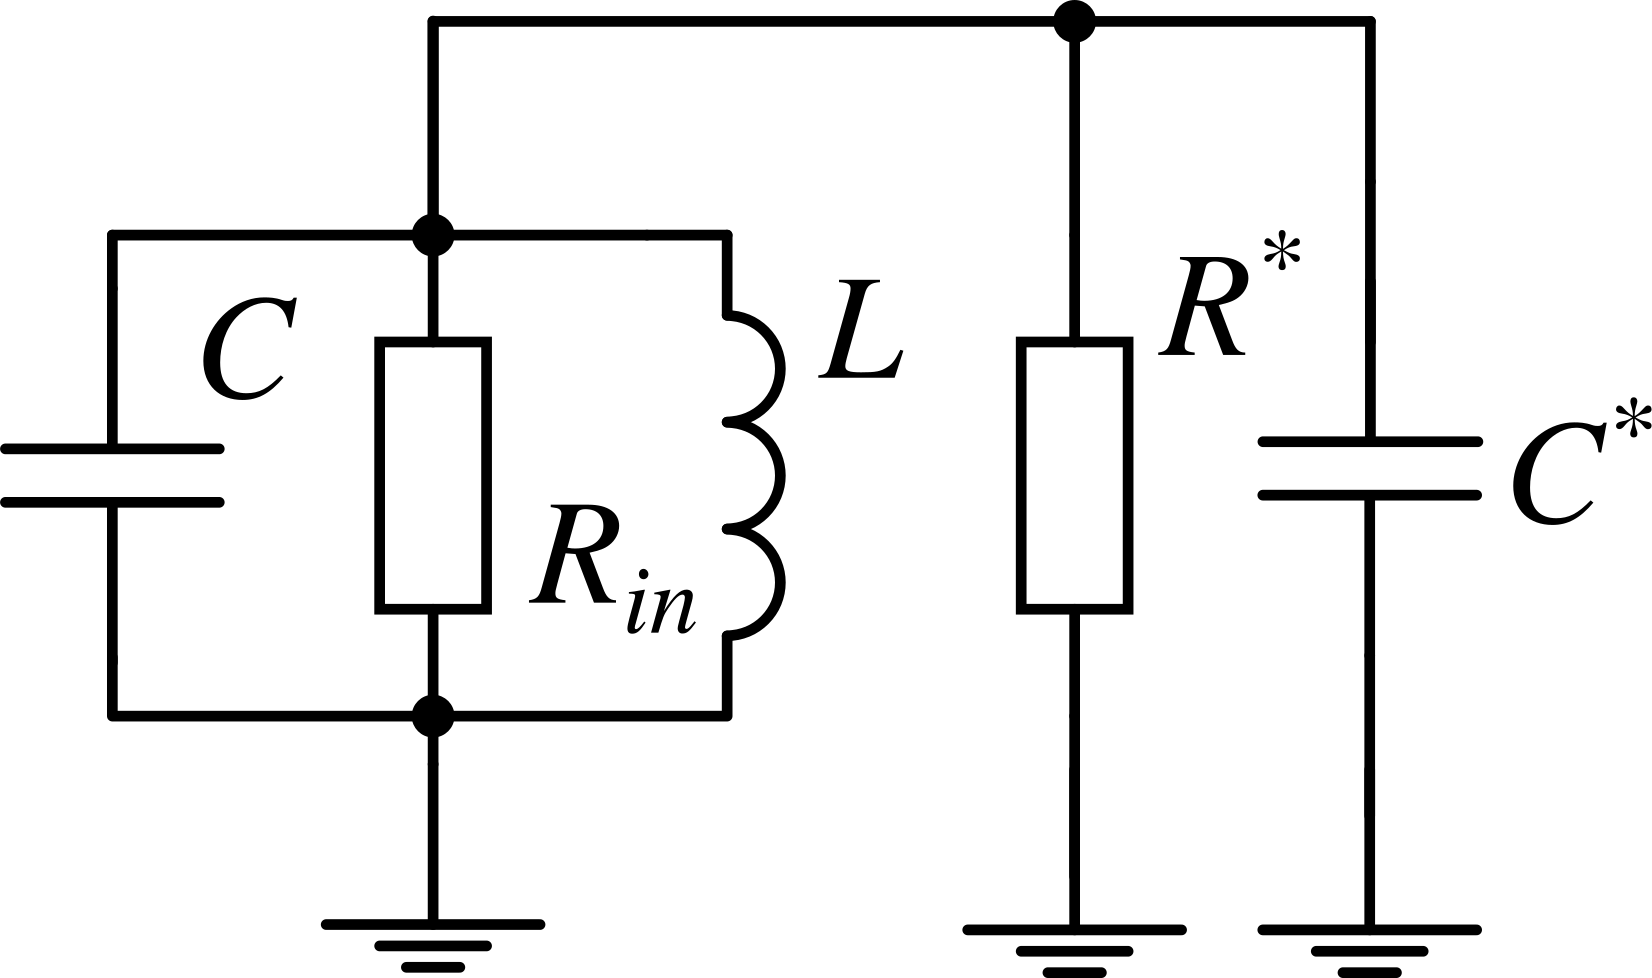
\includegraphics[width=0.9\textwidth]{resonator_equiv}
\caption{Norton equivalent of (a).}
\end{subfigure}

\caption{Equivalent circuit for a $\lambda/4$ TLR, capacitively coupled to the transmission line near resonance.}
\label{fig:resonator_equiv}
\end{figure}

A common way of measuring a resonator is to couple it capacitively to an external transmission line. The coupling on the equivalent scheme of the circuit is represented as $C_\kappa$, as depicted in \autoref{fig:resonator_equiv}~(a). An infinite/properly terminated transmission line can be represented as a single resistance of $Z_0$ Ohms, where $Z_0$ is the line's wave impedance; thus, two such resistances are added to the both sides of the resonator circuit. The resonators are of $\lambda/4$ type, so the equivalent for each of them is a parallel RLC oscillator (see below), where $C$ and $L$ are, respectively, its equivalent capacitance and inductance and $R=R_{in}$ characterises the internal dissipation. Its $Q_i  = \omega_0 C R_{in}$ where $\omega_0 = \sqrt{1/LC}$ can be calculated from the definition when no external impedance is connected.
 
The external Q-factor can be derived in a bit more complicated way\cite{Goppl2008}. We can transform the circuit from the \autoref{fig:resonator_equiv}~(a) to explicitly include the external parameters into the internal ones. To do so one needs to convert the series connection of the coupling capacitor and the characteristic impedances into parallel, as done on the \autoref{fig:resonator_equiv}~(b). The $R^*$ and $C^*$ impedances should be chosen in such a way that total impedance of the external circuit is the same as before the transformation:
\begin{align}
R^{*} &= \frac{1+\omega^2 C_\kappa^2 (Z_0/2)^2}{\omega^2 C_\kappa^2 (Z_0/2)	}, \\
C^{*} &= \frac{C_\kappa}{1+\omega^2 C_\kappa^2 (Z_0/2)^2} \approx C_\kappa\ (\text{in our case}). \label{eq:C_ast}
\end{align}
From this and \autoref{fig:resonator_equiv}~(b) it is simple to write down the expression for the internal, external and loaded quality factors:
\begin{gather}
Q_i =  \omega (C+C^{*}) R_{in}, \\
Q_e = \omega (C+C^{*}) R^{*}, \\
Q_l = \omega (C+C^{*})  \frac{1}{1/R^{*}+1/R_{in}}. \label{eq:Q_l}
\end{gather}
The above expressions readily justify \eqref{eq:qfactor}. The values been used in the simulations are: $C = 350$ fF, $L = 2$ nH, $R_{in}=10^7$ Ohm, $Z_0 = 50$ Ohm. 


\begin{figure}
\centering
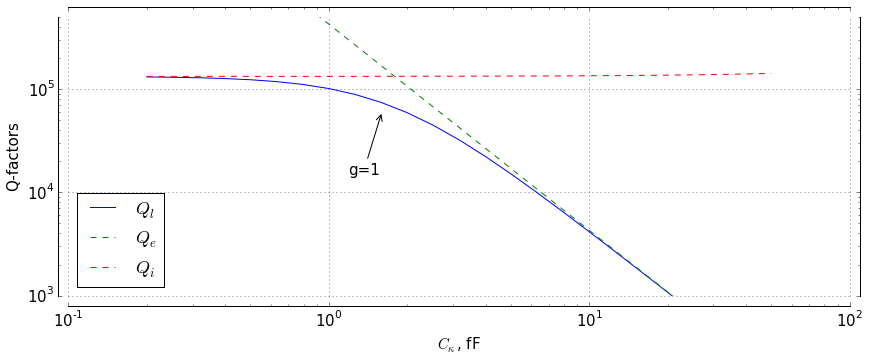
\includegraphics[width=0.9\textwidth]{q-factors}
\caption{Q-factors dependence on $C_\kappa$ according to \eqref{eq:Q_l}.}
\end{figure}


\subsubsection{The lumped-element model of a coplanar waveguide resonator}\label{ssec:LE-model}
A $\lambda/4$ coplanar waveguide (CPW) resonator near a resonance is equivalent to a lumped-element parallel resonance circuit, as in \autoref{fig:resonator_equiv}. $L$ and $C$ for the lumped-element models of CPW resonators are bound not only by the resonance frequency condition $\omega_0 = 1/\sqrt{LC}$ but also by the geometry of the waveguide or, in other words, $C^\prime$ and $L^\prime$ -- the transmission line capacitance and inductance per unit length. To show this, one would write down the impedance of the CPW resonator near its resonance frequency $\omega_0$ and compare it to the lumped-element one's\cite{pozar2012}. Such comparison leads to the following expressions:
\[
R_{in} = \frac{Z_0}{\alpha l}, \quad C = \frac{\pi}{4\omega_0 Z_0},
\]
where $l$ is the resonator length, $Z_0 = \sqrt{L^\prime/C^\prime}$ is the wave resistance and $\alpha$ is the decay constant of the line. Then the resonance condition for the wavelength ($\lambda = 4 l$) is used along with the phase velocity expression $v_{ph} = 1/\sqrt{L^\prime C^\prime}$:
\[
\omega_0 = \frac{2\pi v_{ph}}{\lambda} =  \frac{\pi \, v_{ph}}{2 l} \Rightarrow  C = \frac{C^\prime l}{2}.
\]
For the inductance one can use $L = 1/\omega_0^2 C = 8 l\, L^\prime/\pi^2$. Finally, the expressions for $C^\prime$ and $L^\prime$:
\[
C^\prime = 4\varepsilon_0\varepsilon_{eff} \frac{K(k_0)}{K(k_0^\prime)},\quad
L^\prime = \frac{\mu_0}{4} \frac{K(k_0^\prime)}{K(k_0)},
\]
where $K(x)$ is the complete elliptic integral of the first kind, $\varepsilon_{eff} = \frac{1+\varepsilon_{substrate}}{2}$, $k_0 = \frac{W}{W+2G}$ where $W$ is the width of the hotwire and $G$ is the width of the gaps and finally $k_0^\prime = \sqrt{1-k_0^2}$.

\subsection{S-parameters for lines with resonators}

Typically, a microwave device under test (DUT) is tested with a vector network analyser, which measures the scattering matrix (S-matrix) of the DUT. So below we will discuss the S-matrix for two different coupling configurations. Generally, a two-port DUT can be drawn like in \autoref{fgeneral2port}. For such system it is possible to calculate different 2 by 2 matrices, which bind together voltages and currents on the ports 1 and 2. S-matrix also has 4 values, named S-parameters.

\begin{figure}[h]
\centering
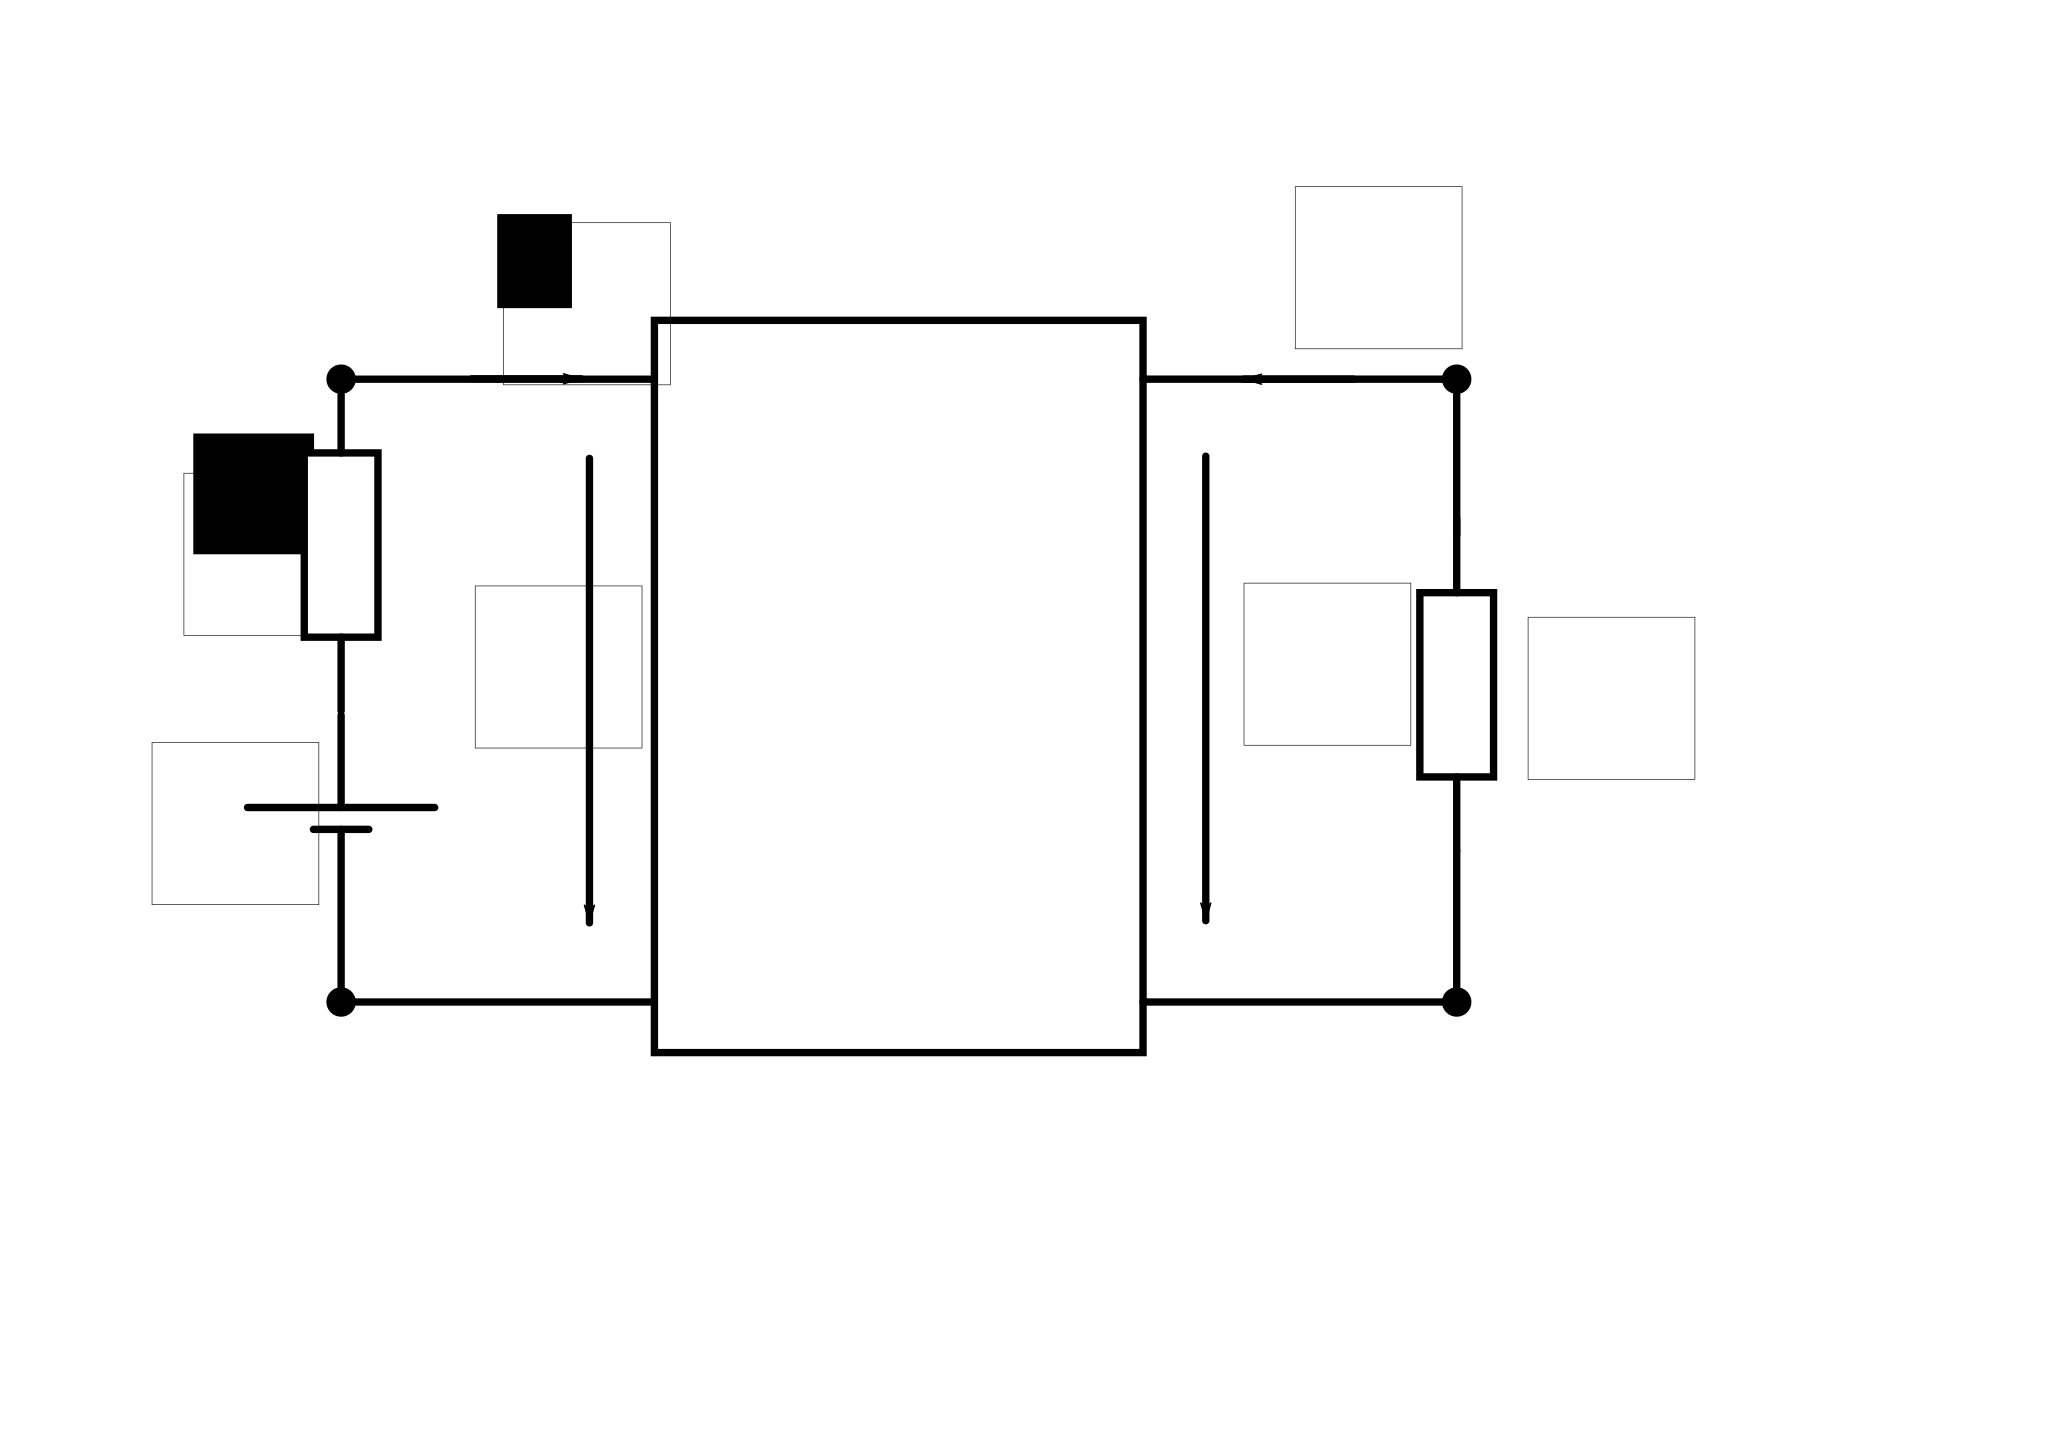
\includegraphics[width=0.5\textwidth]{tl_scheme_general}
\caption{A scheme for the two-port network.}
\label{fgeneral2port}
\end{figure}

To calculate S-parameters one needs to treat voltages and currents, which can be calculated from Kirchhoff's laws, as a sum of the incident and reflected components (``+'' corresponds to the incident wave and ``$-$'' to the reflected wave):
\begin{gather*}
V_{1,2} = V_{1,2}^+ + V_{1,2}^- ,\\
I_{1,2} = I_{1,2}^+ + I_{1,2}^- = \frac{ V_{1,2}^+ - V_{1,2}^- }{Z_0},
\end{gather*}
where the difference in the second expression arises from telegrapher's equations. Solving these with respect to incident and reflected components, one can get
\begin{equation*}
V_{1,2}^\pm = \frac{1}{2}(V_{1,2} \pm Z_0 I_{1,2}).
\end{equation*}
From this, finally, S-parameters are defined:
\begin{equation}
\rbrkt{\begin{matrix}
V_1^- \\
V_2^-
\end{matrix}} = 
\rbrkt{\begin{matrix}
S_{11} & S_{12} \\
S_{21} & S_{22}
\end{matrix}}
\rbrkt{\begin{matrix}
V_1^+ \\
V_2^+
\end{matrix}}.
\label{eq:S_def}
\end{equation}
However, it's often more convenient to use indirect methods of calculating S-parameters, for example, to extract them from $ABCD$-matrix.




\subsubsection{Notch (shunting) design}
For a notch design one can treat the resonator as a shunt in the transmission line as in \autoref{fig:shunted_tl}. Except than by the definition \eqref{eq:S_def} there are two other ways to calculate the S-matrix. First one is intuitive but is not valid for every configuration. Transmission and reflection parameters are defined\cite{Kiselev2013} below (the second formula is valid only for the ``shunt'' configuration, no series elements are allowed in the line):
\begin{gather}    
\Gamma = \frac{Z_{eff} - Z_{0}}{Z_{eff} + Z_{0}} = S_{11} = S_{22}, \label{eGamma}\\
T = \frac{2Z_{eff}}{Z_{eff}+Z_0} \overset{!}{=} S_{21} = S_{12}, \label{eT}
\end{gather}
where $Z_{eff} = Z_0 || Z_{shunt}$, $Z_{shunt} = \frac{1}{i\omega C_\kappa} + 1/i\omega C||R_{in}||i\omega L$ and the equalities between S-parameters hold due to the symmetry.
\begin{figure}[h]
\centering
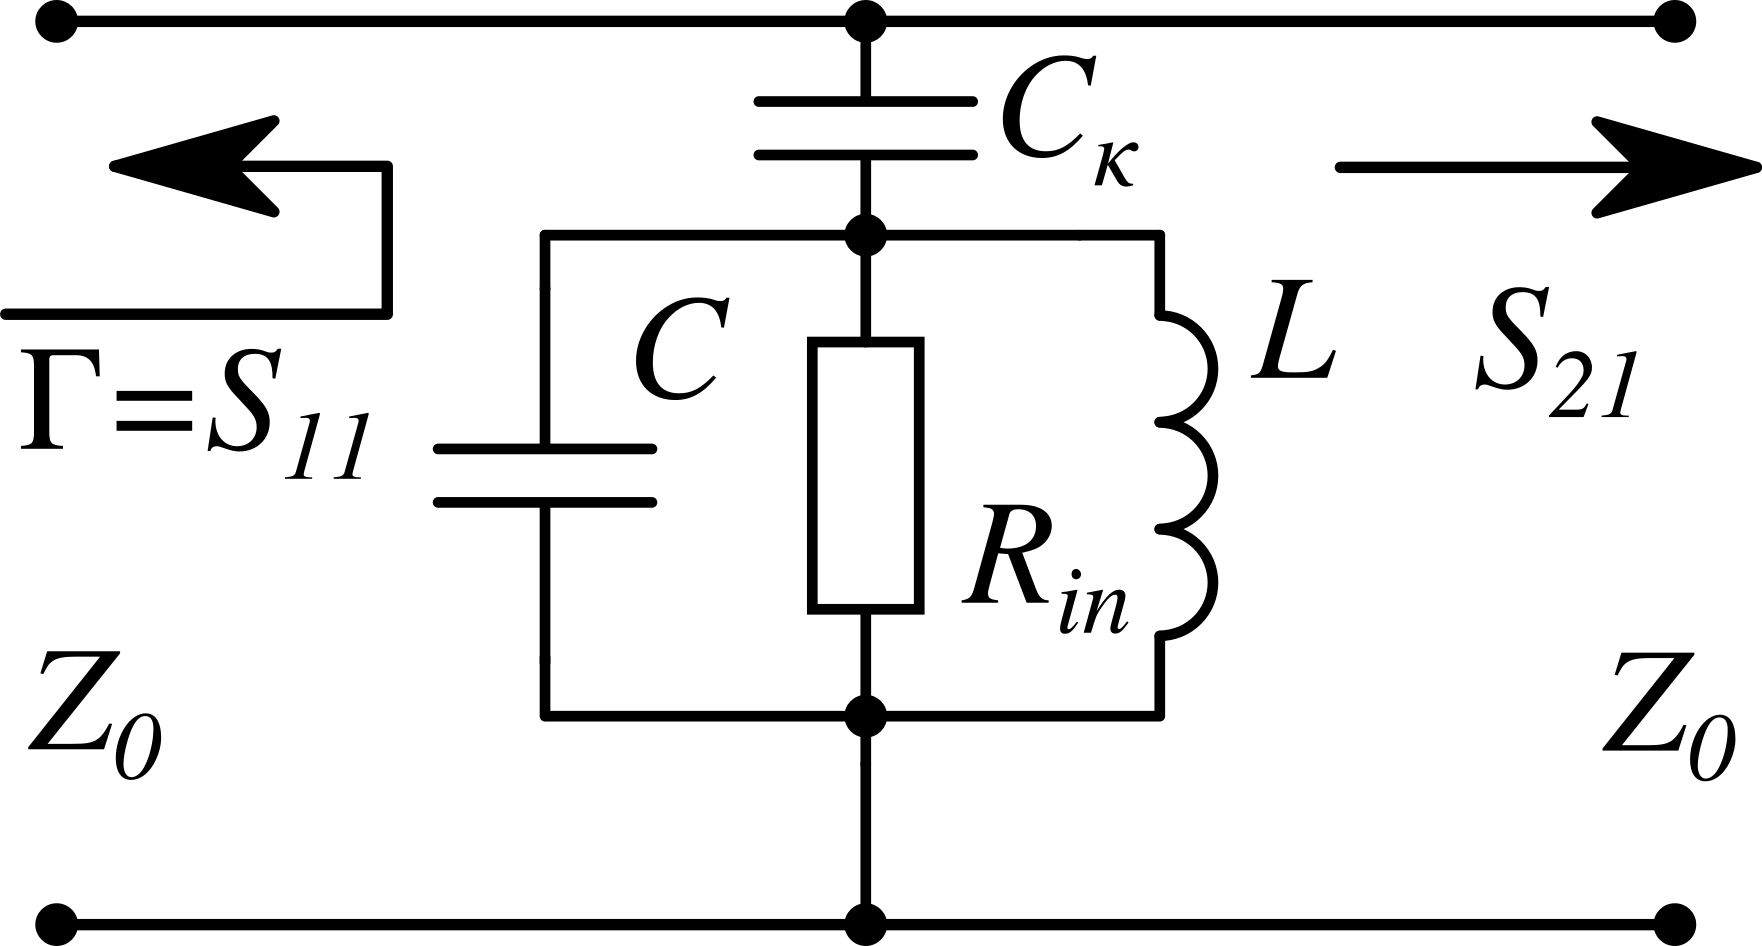
\includegraphics[width=0.5\textwidth]{tl_scheme}
\caption{The shunted transmission line. This is \autoref{fig:resonator_equiv}~(a)  from the observer's point of view.}
\label{fig:shunted_tl}
\end{figure}
\begin{figure}[h]
\centering
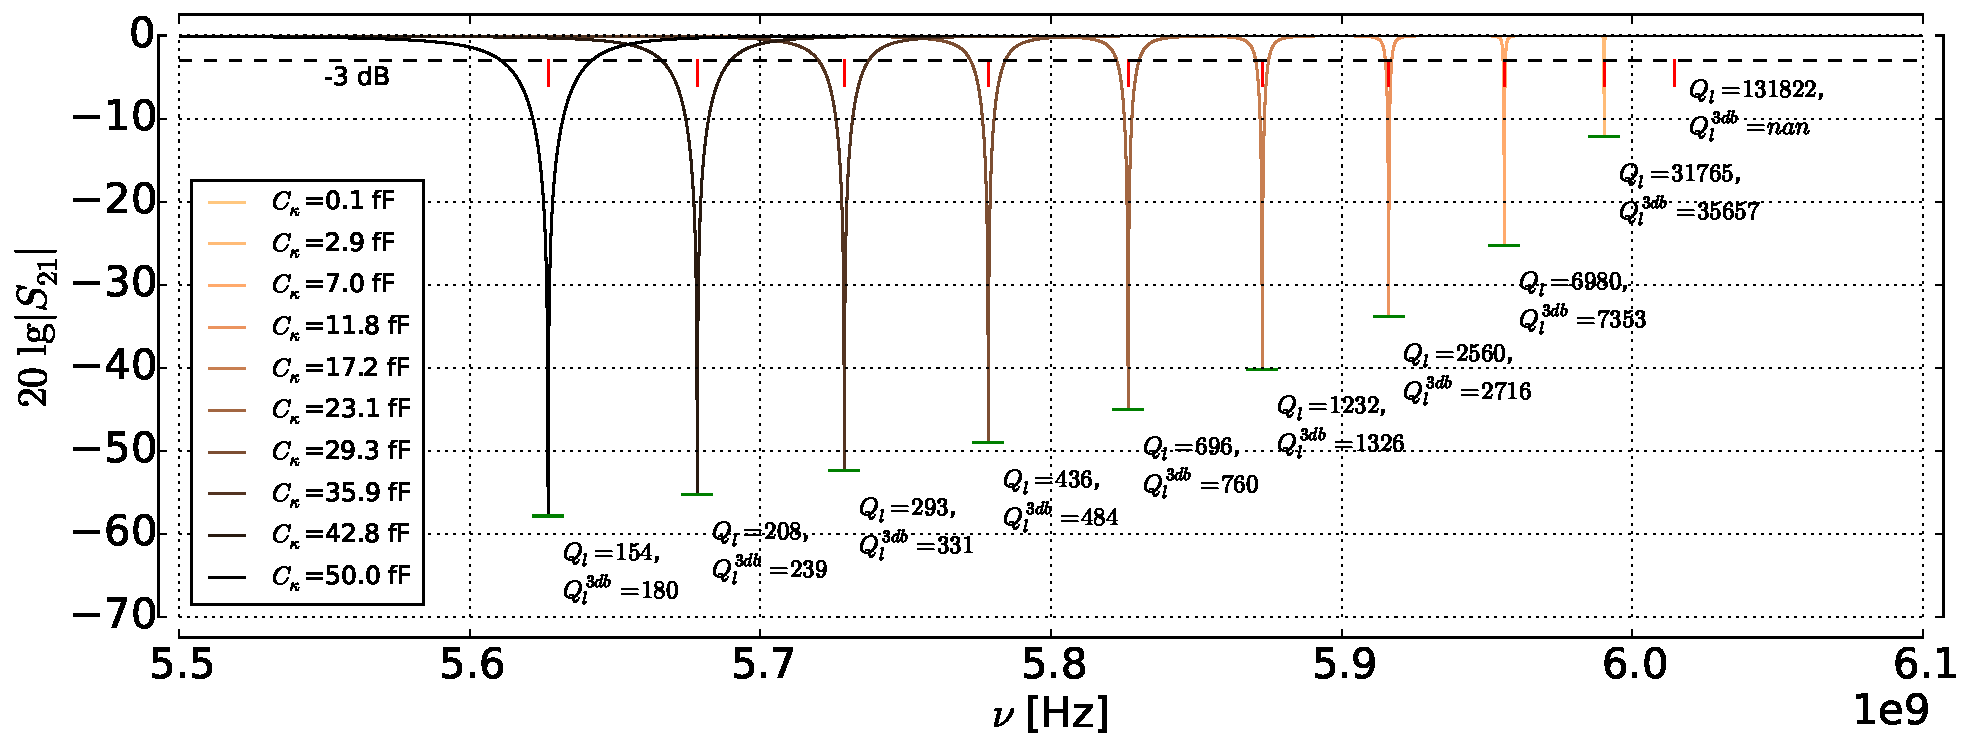
\includegraphics[width=0.99\textwidth]{S21s}
\caption{ $|S_{21}|$ parameters from \eqref{eq:S21} for different coupling strengths. The loaded quality factors are calculated with \eqref{eq:Q_l} and with the ``3db''-method. The red dashes show the values of expression $\sqrt{1/L(C+C_k)}$ according to \autoref{fig:resonator_equiv}~(b), the green ones show the theoretically predicted depths.}
\label{fig:S21s}
\end{figure}

Another way is to calculate $ABCD$ matrix or impedance matrix and convert it to the S-matrix with corresponding formulae\cite{pozar2012}. In the ``shunted'' case from both this approaches the simplified expressions for the S-parameters follow:
\begin{gather}
S_{11} = -\frac{Z_0}{1 + 2Z_{shunt}/Z_0} = S_{22}, \\
S_{21} = \frac{1}{1+Z_0/2Z_{shunt}} = S_{12}. \label{eq:S21}
\end{gather}
The second expression is plotted in \autoref{fig:S21s} along with the loaded quality factors calculated with \eqref{eq:Q_l} and with the ``3db''-method ($Q_L \approx \omega_0/\Delta\omega_{3db}$). It can be seen that with increase of capacitance resonance frequency and $Q_l$ decrease, which is expected according to \autoref{fig:resonator_equiv}~(b) and \eqref{eq:C_ast}.

In \autoref{fig:S21s} the resonance frequencies calculated from the equivalent circuit in \autoref{fig:resonator_equiv}~(b) are shown along with the analytically calculated depths of the peaks:
\begin{equation}
\min_f |S_{21}| = \frac{2 L \left(C + C_{\kappa}\right)}{\sqrt{C_{\kappa}^{2} L Z_{0}^{2} \left(C + C_{\kappa}\right) + \left(2 (C+C_\kappa) L + C_{k}^{2} R_{in} Z_{0} \right)^{2}}}.
\end{equation}

\subsubsection{Embedded (series) design}

For the embedded resonator it's possible to draw a similar equivalent circuit as for the ``shunt'' design\cite{Goppl2008}. It is depicted in \autoref{fseries_tl}. 

\begin{figure}[h]
\centering
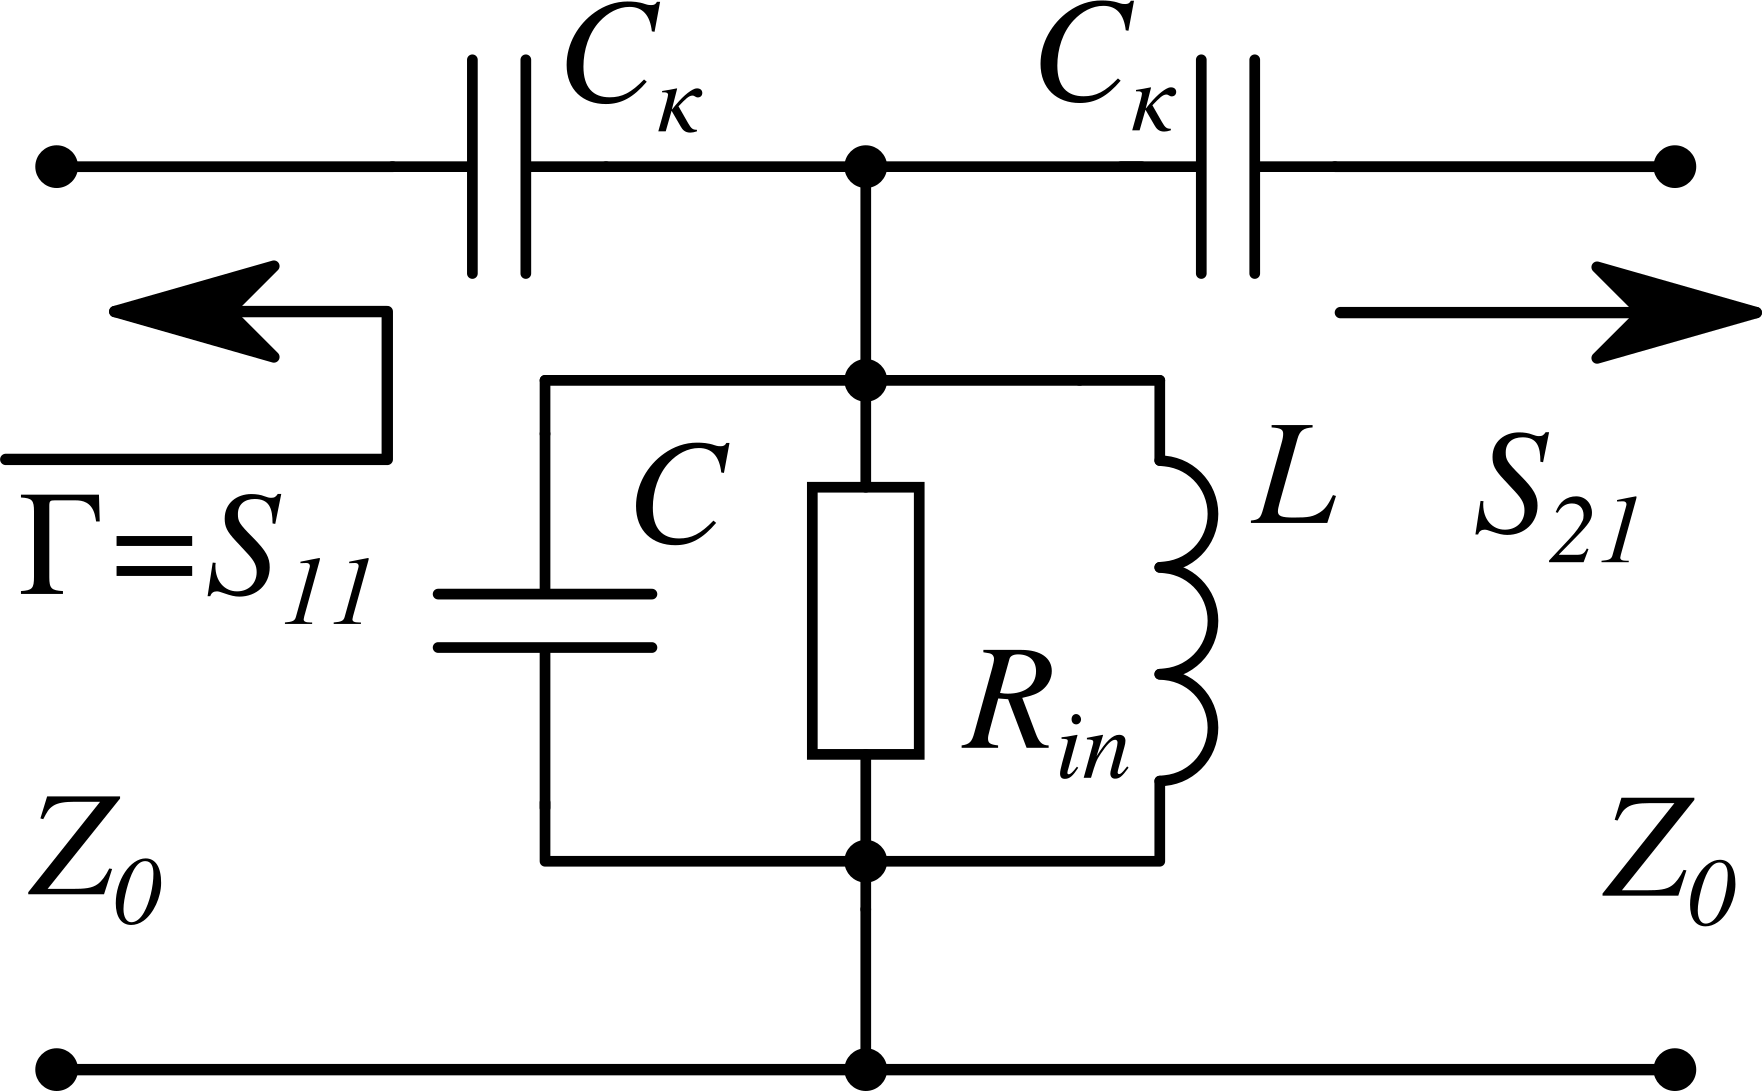
\includegraphics[width=0.5\textwidth]{tl_scheme_series}
\caption{The equivalent circuit for the embedded resonator.}
\label{fseries_tl}
\end{figure}
\begin{figure}[h]
\centering
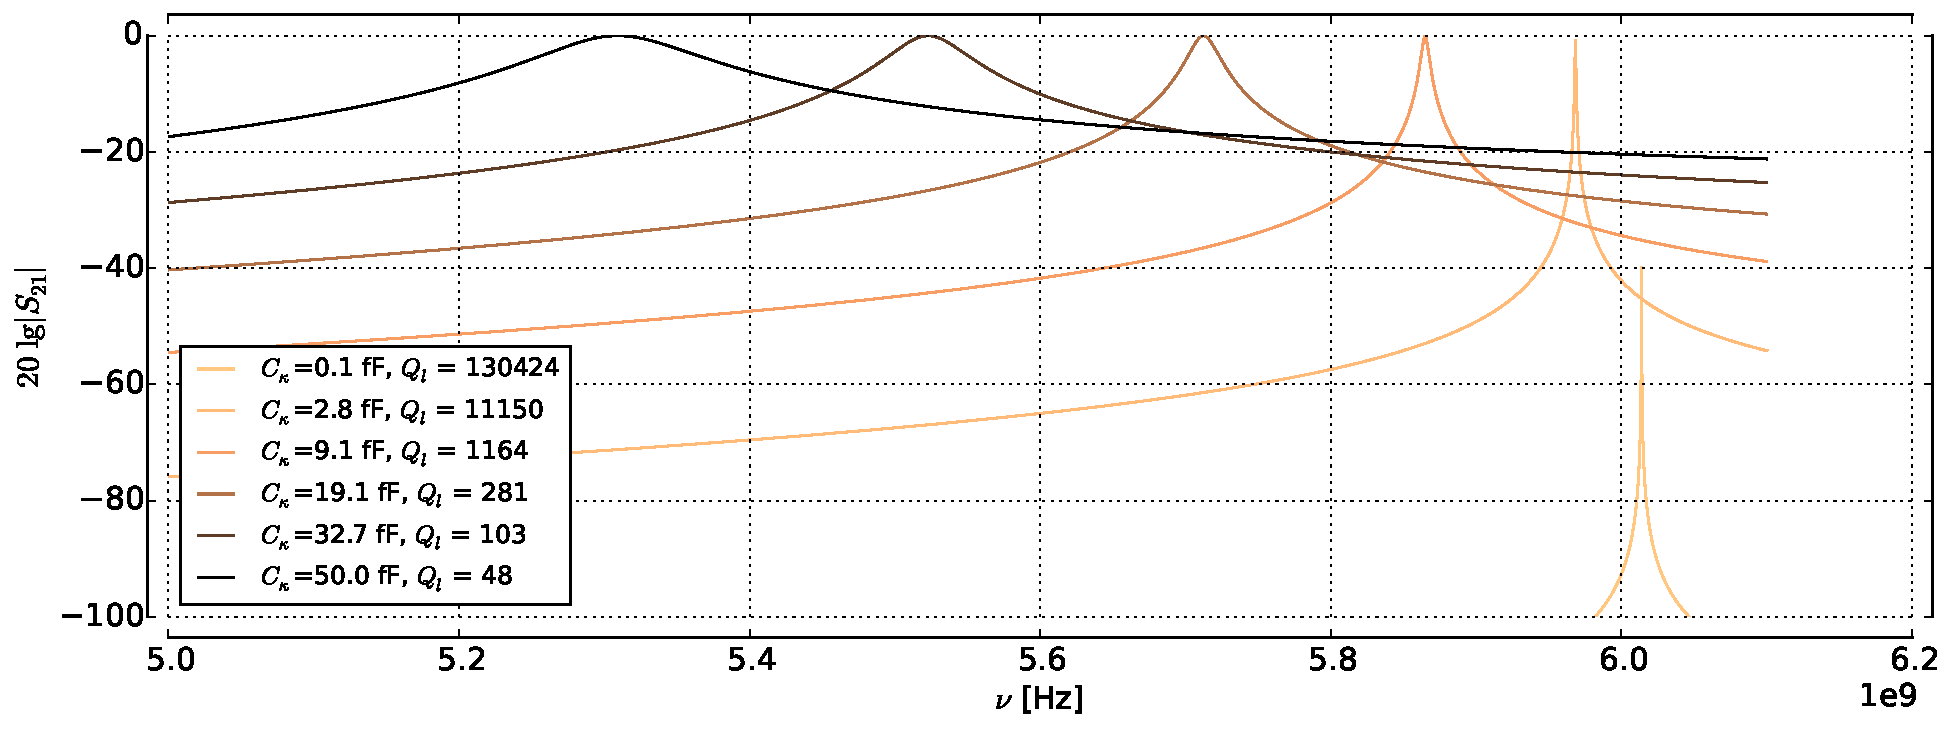
\includegraphics[width=0.9\textwidth]{S21s_series}
\caption{$S_{21}$ for the series configuration. Loaded Q-factors were calculated  via analytic expression similar to \eqref{eq:Q_l}.}
\label{fS21s_series}
\end{figure}

For this kind of connection of the resonator to the transmission line \eqref{eT} is now not valid (however, \eqref{eGamma} still holds). To calculate transmission in this case one may find the transmission matrix and then convert it to the S-matrix or use Kirchhoff's laws and \eqref{eq:S_def}. For studied case one can get the following $ABCD$-matrix\cite{pozar2012}
\begin{equation}
\hat T = \rbrkt{\begin{matrix}
A & B \\
C & D
\end{matrix}} = \rbrkt{\begin{matrix}
1 + \frac{1/i\omega C_\kappa}{Z_{res}} & 2/i\omega C_\kappa - \frac{\omega^2 C_\kappa^2}{Z_{res}} \\
1/Z_{res} &  1 + \frac{1/i\omega C_\kappa}{Z_{res}} 
\end{matrix}},
\end{equation}
where $Z_{res} = R_{in}||i\omega L || 1/i\omega C$. The corresponding $S_{21}$ is plotted in \autoref{fS21s_series}, calculated as\cite{pozar2012} 
\begin{equation}
S_{21} = \frac{2}{A+B/Z_0 +CZ_0 + D}.
\end{equation}

\subsection{Time-resolved response}

As soon as the spectral characteristics of the resonator are established is is possible to calculate it's response when a pulse of finite width is applied to it. The shape that the pulse will have after it has interacted with the resonator is important when pulsed readout is considered in time-resolved qubit measurements. 

In this section we will only discuss the notch-type resonator and only the transmission of the pulses; however, the numerical method that will be used can be straightforwardly extended to other cases. It consists of three steps: calculate the discrete Fourier transform (DFT) for the input pulse, multiply it by the required complex S-parameter for each frequency (negative and positive frequencies should be multiplied in the same way), and finally perform the inverse discrete Fourier transform. 

We will use the following expression for the complex $S_{21}$ of an ideal notch-type resonator\cite{probst2015}:

\[
S_{21} (\omega)= 1 - \frac{Q_l/Q_e}{1 + 2 i Q_l (\omega/\omega_0 - 1)}.
\]

Then we perform the following operation on the input rectangular pulse $x(t)$ to obtain the transformed signal $x'(t)$:
\[
x'(t) = \frac{1}{2\pi}\int\limits_{-\infty}^{+\infty} e^{i\omega t} {S_{21}(-\omega_r, \omega)}S_{21}(\omega_r, \omega)\int\limits_{-\infty}^{+\infty} e^{-i\omega t}x(t) \diff t \diff \omega.
\]

Using DFT this procedure becomes a little bit more tricky as it requires careful tracking of the indices and asymmetries that emerge from discreteness. The results of such calculation are presented in \autoref{fig:res_pulse} and \autoref{fig:ro_pulse_diff}. 


\begin{figure}
\includegraphics[width=\textwidth]{resonant_pulse}
\caption{Calculated shape of the resonant pulse transmitted through the notch-type resonator ($f_0 = 6$ GHz, $Q_e=6 \cdot 10^3,\ Q_i = 10^4$). Due to very high frequency of the input pulse only it's envelope extracted using Hilbert transform is presented. Output pulse is obtained by simulating a downconversion: the UHF pulse after the resonator was multiplied by a sine wave detuned by low intermediate frequency of 50 MHz and then filtered with a digital 100 MHz low-pass filter. This procedure is very useful as it allows to visualize the phase of the UHF signal and, moreover, exactly models that what occurs in experiment.}
\label{fig:res_pulse}
\end{figure}

\autoref{fig:res_pulse} shows what happens with a rectangular pulse with resonant carrier frequency when it comes through the notch-type resonator. The output pulse has a peculiar shape that can be divided in time into three parts: the ``ring-up'' part, the steady state part, and the ``ring-down'' part. The first part is an exponent-like transient with rate determined by both $Q_e$ and $Q_i$, the steady state part  determines the amplitude and phase of the transmitted  signal in the continuous wave measurements, and the third part is simply an exponential decay of the excitation inside the resonator with rate $\kappa = \omega_0/Q_l$ at frequency $\omega_0$. Additionally, the shape of the pulse does not depend on power; however, the steady-state amplitude of the wave inside it (or the number of photons in the quantum limit) does. So in the experiment length of the pulses or the spacing between them do not define the number of photons inside the resonator as long as they are long enough to drive the resonator into the steady state.

\begin{figure}[h!]
\includegraphics[width=\textwidth]{ro_pulse_difference}
\caption{Simulated response for slightly off-resonant interaction (as in dispersive readout). The input pulses were identical, but the resonance frequency was either higher (orange) or lower (blue) than their carrier frequency. Here pulse carrier was 6 GHz, and resonator frequencies were 6.0005 GHz and 5.9995 GHz, respectively. The difference between instantaneous phases calculated from Hilbert transform is also presented.}
\label{fig:ro_pulse_diff}
\end{figure}

\begin{figure}[h!]
\includegraphics[width=\textwidth]{ro_pulse_fourier}
\caption{Separate DFTs for two different pulse parts. Same two resonator frequency cases as in \autoref{fig:ro_pulse_diff} are displayed in blue and orange, respectively. Notice that the ``ring-down'' parts are close to resonator frequency in contrast to the ``ring-up'' and steady state parts which are closer to the pulse carrier frequency.}
\end{figure}

In \autoref{fig:ro_pulse_diff} two output pulses obtained from the same input rectangular pulse are presented for two different cases of resonance frequency above and below the pulse carrier frequency. It can be seen that during the first 100 ns the two output pulses are nearly identical in their amplitude and phase. Then, gradually, the phase difference between the pulses begins to accumulate until it reaches saturation in the steady state. Then the ``ring-down'' part begins and the phase difference changes the sign abruptly and then continues to accumulate. This behaviour is due to the fact that, firstly, the resonator has to accumulate the amplitude at least comparable to the amplitude of the incident wave to influence it in any way, i.e., to shift its phase. This is why the first part is called ``ring-up''. Then it reaches the steady state where the phase difference is constant and equals the value one would observe on a vector network analyser. Finally, the phase difference between the ``ring-down'' parts of the two pulses is caused simply by the difference between the resonator frequencies (after the end of the pulse the resonator experiences free oscillations).



\newpage

\section{Cirquit QED with transmon qubits}\label{sec:cQED}

\subsection{Transmon}

Before turning to the circuit QED with transmons, it is necessary first to describe the transmon itself. This type of qubit has been introduced\cite{Koch2007} in 2007 by J. Koch et al., and since then was used extensively in many groups around the world. 

A transmon is a Cooper pair box where the Josephson junction (JJ) capacitance is extended with a shunt capacitor inserted in parallel with the junction (see \autoref{fig:cpb-transmon-floating_transmon}~(a),(b)) which leads to the reduction of the capacitive energy of the circuit. The reason for this modification is that it exponentially suppresses the \textit{charge dispersion}, that is, the dependence of the energy levels of the qubit on the induced charge, while maintaining a sufficient anharmonicity of the circuit. This means that such qubits are becoming immune to dephasing from the charge noise ubiquitous on the chip due to dipole defects. Recently, flux qubits with increased coherence due to a capacitively shunted smaller junction were also demonstrated\cite{yan2015}.

\begin{figure}[h!]
\centering
\includegraphics[width=\textwidth]{cpb-transmon-floating_transmon}
\caption{Transition from a charge qubit to a transmon. Colours and Greek letters denote the degrees of freedom of the systems. \textbf{(a)} Cooper pair box which is simply a JJ connecting a small superconducting island with the ground. \textbf{(b)} Transmon which is different from (a) just by the additional shunting capacitor $C_{sh}$ in parallel to the junction, i.e., larger island with dominating capacitance to the ground. \textbf{(c)} Floating transmon, a variation of the design (b) which is not connected to the ground and has two superconducting islands. The charge is saved in the system, so the two degrees of freedom can be reduced to one, $\phi_q - \zeta_q$.}
\label{fig:cpb-transmon-floating_transmon}
\end{figure}

Two versions of the transmon qubits exist (see \autoref{fig:cpb-transmon-floating_transmon}~(b),(c)). The first has a single superconducting island which has some large (compared to the JJ) capacitance to the ground, and the second has two islands forming a capacitor. These two versions are exactly the same conserning the energy structure given that their electrical parameters are the same; however, the second type does not require the ground plane, and thus can be used in 3D waveguides or waveguide resonators\cite{paik2011}. In the original transmon paper\cite{Koch2007} the second form was presented, and the first form was not mentioned. This led to the wide spread of the two-island transmons both in 3D and planar architectures which had many different shapes of the capacitors. For planar cQED this was an unncesessary complication as the calculation of the coupling for such qubits is much more complicated (see Appendix B of the Koch's paper). The transmons of the first type (embedded in the ground plane) became popular after the work\cite{barends2013} by the group of J. Martinis where they have demonstrated a coherent transmon with a single superconducting island.

Below we discuss the quantum mechanics of a transmon of the first type, as long as this is the type that was investigated in the experimental part. But, until we turn to coupling calculation the results for the two-island qubits are exactly the same. First of all, the Hamiltonian of the system depicted in \autoref{fig:cpb-transmon-floating_transmon}~(b) is written down:
\begin{equation}
\hat H_{tr} = 4E_C \hat n^2 - E_J\cos \hat \varphi,
\label{eq:tr_ham}
\end{equation}

where $E_C = e^2/2C_\Sigma$, $C_\Sigma = C_J+C_{sh}$, $E_J = I_c \hbar/2e$ is the standard Josephson energy, $\hat n$ is the number operator of excess cooper pairs on the island and $\hat \varphi$ is the phase difference operator across the junction (equal to the phase operator $\hat \phi$ of the single island of to the phase difference operator between two islands\cite{Devoret1995}). The phase-dependent part of this Hamiltonian can be transformed into charge representation. From the Euler's formula $\cos \hat \varphi = (e^{i\hat\varphi} + e^{-i\hat\varphi})/2$, the fact that $n$ and $\varphi$ are conjugate variables, i.e., $\braket{\varphi}{n} = \psi_n(\varphi) = e^{i n \varphi}$, the series expansion of the exponent and decomposition of the unity operator $\mathbbm{\hat 1} = \int \diff \varphi \ket{\varphi}\bra{\varphi}$, we obtain
\[
\begin{aligned}
e^{\pm i \hat \varphi}\ket{n} &= \sum_n \frac{\pm i\varphi}{k!}\ket{n} = \int \diff \varphi \sum_k \frac{(\pm i)^k \hat\varphi^k \ket{\varphi}}{k!}\braket{\varphi}{n}\\
&=  \int \diff \varphi e^{\pm i\varphi} e^{i n \varphi} \ket{\phi} = \int \diff \varphi \ket{\varphi}\braket{\varphi}{n\pm1}\\
&= \ket{n\pm1}.
\end{aligned}
\]
With this equality and the orthogonality of the $\ket{n}$ states, we can construct the operator $\cos\hat\varphi$:
\[
\cos\hat\varphi = \frac{1}{2}\sum_n\sbrkt{\ket{n+1}\bra{n} + \ket{n-1}\bra{n}}.
\]
This representation allows straightforward numerical solution of different eigenproblems with transmons in the simple matrix form.

Another point that should be mentioned is the possibility of replacement of the single JJ in the transmon by a SQUID. This makes the transmon's energy spectrum tunable by external magnetic flux flowing through the loop of the SQUID. The dependence of the Josephson energy on the flux is then described by the following expression\cite{Koch2007}:
\[
E_J(\Phi_{ext}) = (E_{J1} + E_{J2})\cos\rbrkt{\pi\frac{\Phi_{ext}}{\Phi_0}}\sqrt{1+d^2\tan^2\rbrkt{\frac{\pi\Phi_{ext}}{\Phi_0}}},
\]
where $d = \frac{E_{J1} - E_{J2}}{E_{J1} + E_{J2}}$ is the SQUID asymmetry. In this case the flux value which provides the largest possible $E_J$ (for example, $\Phi_{ext} = 0$) is called \textit{sweet spot} since in it the transmon is maximally insensitive to the flux noise.


\subsection{Transmon eigenproblem}\label{sec:tr_eigen}

\begin{figure}
\centering
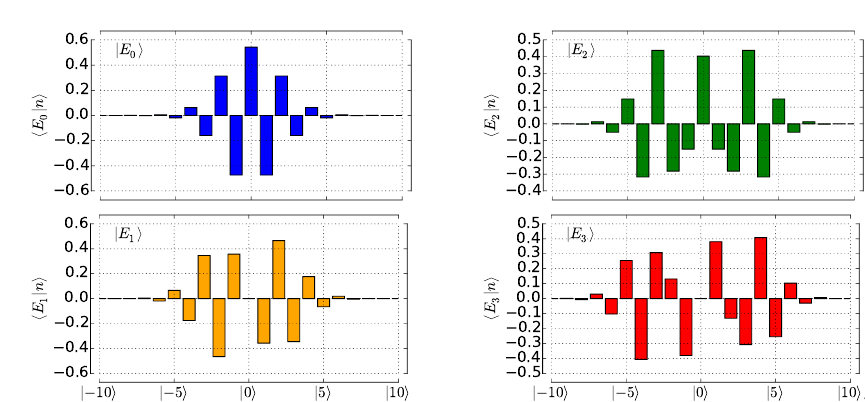
\includegraphics[width=\textwidth]{tr_CPD}
\caption{Eigenstates in charge representation for first four energy levels of the transmon. Note how the parity of the states is switched from even to odd and back with increasing $m$. This behaviour is the same for higher levels, too.}
\label{fig:tr_states}
\end{figure}

In this section the solution of the problem $\hat H_{tr} \ket{m} = E_m \ket{m}$ will be discussed. That is, it is necessary to find the eigenenergies and eigenstates of the transmon. As long as the transmon can be considered as a slightly anharmonic quantum oscillator, it is possible to calculate its energy spectrum perturbatively by expanding the cosine function in the \eqref{eq:tr_ham} up to the fourth order term. This approach leads\cite{Koch2007} to the following energy structure (up to a constant offset):
\begin{equation}
E_m = m \sqrt{8E_J E_C} -\frac{E_C}{12}(6m^2+6m),
\label{eq:tr_levels}
\end{equation}
Additionally, numerically obtained eigenstates in charge basis for $m=1..4$ are shown in \autoref{fig:tr_states}. From this expression we can notice already that each subsequent transition frequency $\omega_{n-1,n}$ is reduced by the value of $n E_C/\hbar$, so we define the \textit{anharmonicity} $\alpha = -E_C/\hbar$ of the transmon (in frequency units) which makes its level structure different from the harmonic oscillator's, hence the name.

\begin{figure}
\centering
\includegraphics[width=\textwidth]{n_mes}
\caption{Some of the matrix elements of the $\hat n$ operator. Note the linear decay of the matrix elements in the log scale over ``distance'' between states which means exponential suppression of the transition rates between them. This suppression is much more pronounced for low initial states than for the higher ones. Single-photon transitions between states of same parity are forbidden and because the corresponding matrix elements are zero.}
\label{fig:n_mes}
\end{figure}


For convenience, below we will denote first energy levels as $g,e,f,d$. We will look at the expression \eqref{eq:tr_levels} in detail. We need to find out what transition frequencies near transition $ge$ ($\omega_{ge} = E_e - E_g = \sqrt{8E_J E_C} - E_C$) can be observed in the experiment, especially in case of a non-zero thermal population of the first excited state and including multiphoton transitions. 

The operator which is responsible for transmon excitation in case of capacitive coupling to the driving field (classical or quantized) is simply proportional to $\hat n$\cite{Koch2007}. So, to determine what transitions are allowed, it is very useful to look at the parity of the eigenstates of the transmon in $n$-representation in \autoref{fig:tr_states} and to recall that $\hat n$ is itself odd. Obviously, $\hat n$ can not induce transitions between states of same parity in a single-photon process as long as $\bra{m}\hat n\ket{m+2j} = 0,\ j\in\mathbb{Z}$. Moreover, in general single-photon transitions between distant levels $m\rightarrow m+k$ where $k>1$ are more or less suppressed\cite{Bishop2010} even for the odd $k$ (for large $m$ this may be not exactly true, see \autoref{fig:n_mes} for exact numerically obtained data). 

In \autoref{tab:tr_transitions} first five eigenenergies and frequencies of allowed transitions between them calculated with \eqref{eq:tr_levels} are presented. The frequencies listed there are expected to appear on the spectral data in the experiment, and indeed they may be observed when the excitation power is high enough. We will discuss the oscillator strengths for these transitions calculated from perturbation theory and look at numerical simulations in the \autoref{sec:dynamics} where quantum dynamics of our systems will be studied.

\begin{table}
\centering
\begin{tabular}{l|c}
Level & Energy\\
\hline
$g$ & 0\\
$e$ & $\sqrt{8E_J E_C} - E_C$\\
$f$ & $2\sqrt{8E_J E_C} - 3 E_C$\\
$d$ & $3\sqrt{8E_J E_C} - 6 E_C$\\
$E_4$ & $4\sqrt{8E_J E_C} - 10 E_C$\\
\hline
\end{tabular}\quad
\begin{tabular}{l|c}
Transition & Frequency\\
\hline
$ge$ & $\omega_{ge}$ \\
$gf/2$ & $\omega_{ge} - 0.5 E_C$\\
$ef$, $gd/3$& $\omega_{ge}-E_C$\\
$ed/2$ & $\omega_{ge} - 1.5 E_C$\\
$fd$, $e E_4/3$ & $\omega_{ge}-2 E_C$\\
\hline
\end{tabular}
\caption{Energies and some transition frequencies for first 5 levels of the transmon calculated with \eqref{eq:tr_levels}.}
\label{tab:tr_transitions}
\end{table}

\subsection{Hamiltonian of the transmon-resonator system}

In this section one of the most important concepts in the area of superconducting quantum devices will be reviewed. It is the so-called \textit{circuit QED} or \textit{cQED}, i.e., circuit quantum electrodynamics of cavity quantum electrodynamics in electrical circuts\cite{Blais2004}. The idea of cQED is to couple a superconducting qubit to an electric oscillator (which is usually a mode of a microwave transmission line resonator) to obtain many useful effects such as non-demolition readout\cite{Blais2004}, Purcell decay protection\cite{Koch2007}, coupling of distant qubits\cite{Majer2007}, single photon emission\cite{bozyigit2011}, etc.

With transmon qubits cQED approach is crucial since it is not possible to directly read out the transmon state neither with charge nor with flux based measurement apparatus since transmon eigenstates are electrically and magnetically neutral (at the sweet spot). However, the \textit{dispersive readout}\cite{Blais2004} of such qubits has now been proven to be very effective. Below we will calculate the spectrum of the transmon-oscillator system and find the transmon state-dependent dispersive shifts.

\begin{figure}
\centering
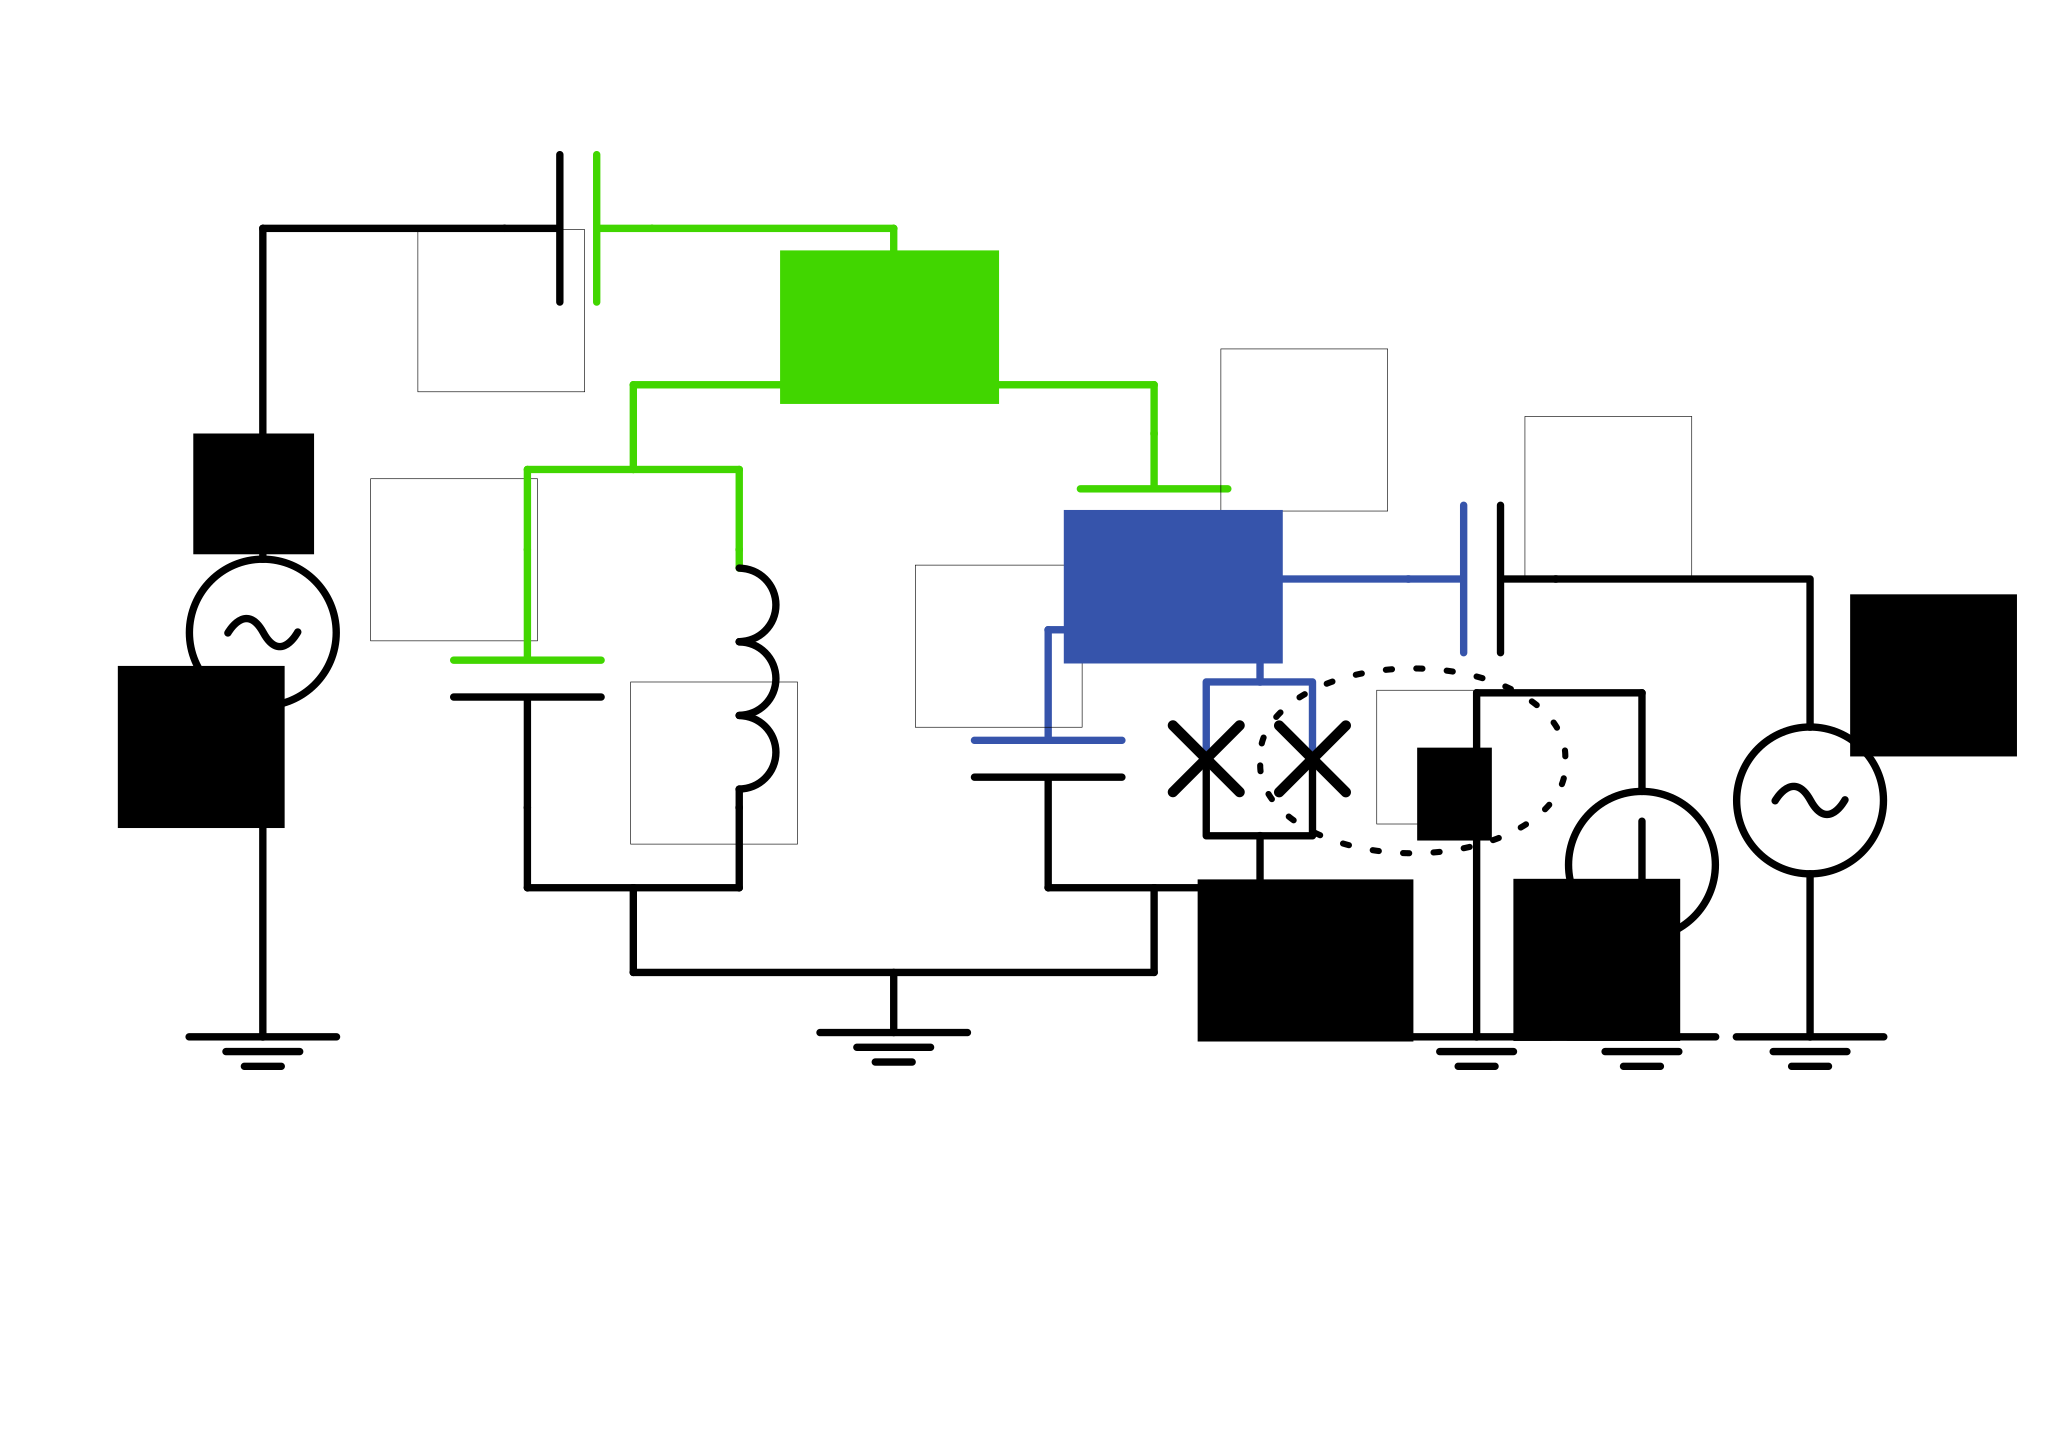
\includegraphics[width=0.8\textwidth]{xmon-resonator}
\caption{Equivalent circuit for coupled system of a tunable transmon qubit and a resonator. Colors show nodes (or branches) containing system's degrees of freedom according to M. Devoret's theory\cite{Devoret1995}.}
\label{fig:xmon-resonator}
\end{figure}

First of all, it is necessary to construct the full Hamiltonian for the transmon-oscillator system depicted in \autoref{fig:xmon-resonator}. We will use the results acquired by Bader\cite{Bader2013} and Koch\cite{Koch2007}. The system under study has two degrees of freedom; one from the resonator and one from the qubit. The coupling between the systems is achieved due to the presence of a capacitor $C_g$ whose energy depends on both degrees of freedom. The Lagrangian of the circuit is then easy to write down, and with some calculations it is possible to obtain as well the quantized Hamiltonian for the compound circuit:

\begin{equation}
\begin{gathered}
\mathcal{\hat H} =  \underbrace{\frac{\hat \phi_r^2}{2 L_r} + \frac{(C_q+C_g) \hat Q_r^2}{2C_*^2}}_\text{resonator} 
+ \underbrace{\frac{(C_g + C_\kappa + C_r) \hat Q^2_q}{2C_*^2} - E_J (\Phi_{ext}) \cos \frac{2e}{\hbar}\hat \phi_q }_\text{qubit}
+ \underbrace{\frac{C_g\hat Q_r \hat Q_q}{C_*^2}}_\text{coupling} = \\
=  \hbar\omega_r\ \hat a^\dag \hat a \otimes \mathbbm{\hat 1}_q \quad (\mathcal{\hat H}_r) \\
+ 4 E_C\ \mathbbm{\hat 1}_r \otimes \hat n^2 - \frac{E_J(\Phi_{ext})}{2}\ \mathbbm{\hat 1}_r\otimes \sum_{n=-\infty}^{+\infty} \ket{n+1}\bra{n} + \ket{n}\bra{n+1} \quad (\mathcal{\hat H}_q) \\
- 2e \frac{C_g}{C_*} \sqrt{\frac{\hbar \omega_r }{2(C_q+C_g)}}\ i(\hat a^\dag - \hat a) \otimes \hat n, \quad (\mathcal{\hat H}_i)
\end{gathered}\label{eq:hamiltonian}
\end{equation}
where 
$$C_*^2 = C_q C_g + C_q C_\kappa + C_g C_\kappa + C_q C_r + C_g C_r, $$
$$\omega_r = 1/\sqrt{L_r C_*^2/(C_q+C_g)}, $$
$$E_C = \frac{(C_g+C_\kappa+C_r)e^2}{C_*^2}, $$
$$E_J(\Phi_{ext}) = E_{J,\Sigma} \cos(\Phi_{ext}/\Phi_0),\ \Phi_{ext} = I_\Phi M.$$
Presuming the coupling is not very strong ($C_g \ll C_q, C_r$) it is possible also to include simple time-dependent driving terms for both subsystems:
\begin{gather}
\mathcal{\hat H}_r^d(t) = \frac{C_\kappa V_\kappa(t)}{C_r + C_\kappa} \hat Q_r \propto f_r(t)\ i(\hat a^\dag - \hat a) \otimes \mathbbm{\hat 1}_q, \notag \\
\mathcal{\hat H}_q^d(t) = \frac{C_e V_e(t)}{C_q + C_e} \hat Q_q \propto f_q(t)\  \mathbbm{\hat 1}_r \otimes \hat n,
\label{eq:driving_q}
\end{gather}
where $f_{q, r} (t)$ are the effective values of the drive magnitudes at time $t$.

\begin{figure}
\centering
\begin{subfigure}[t]{\textwidth}
\centering
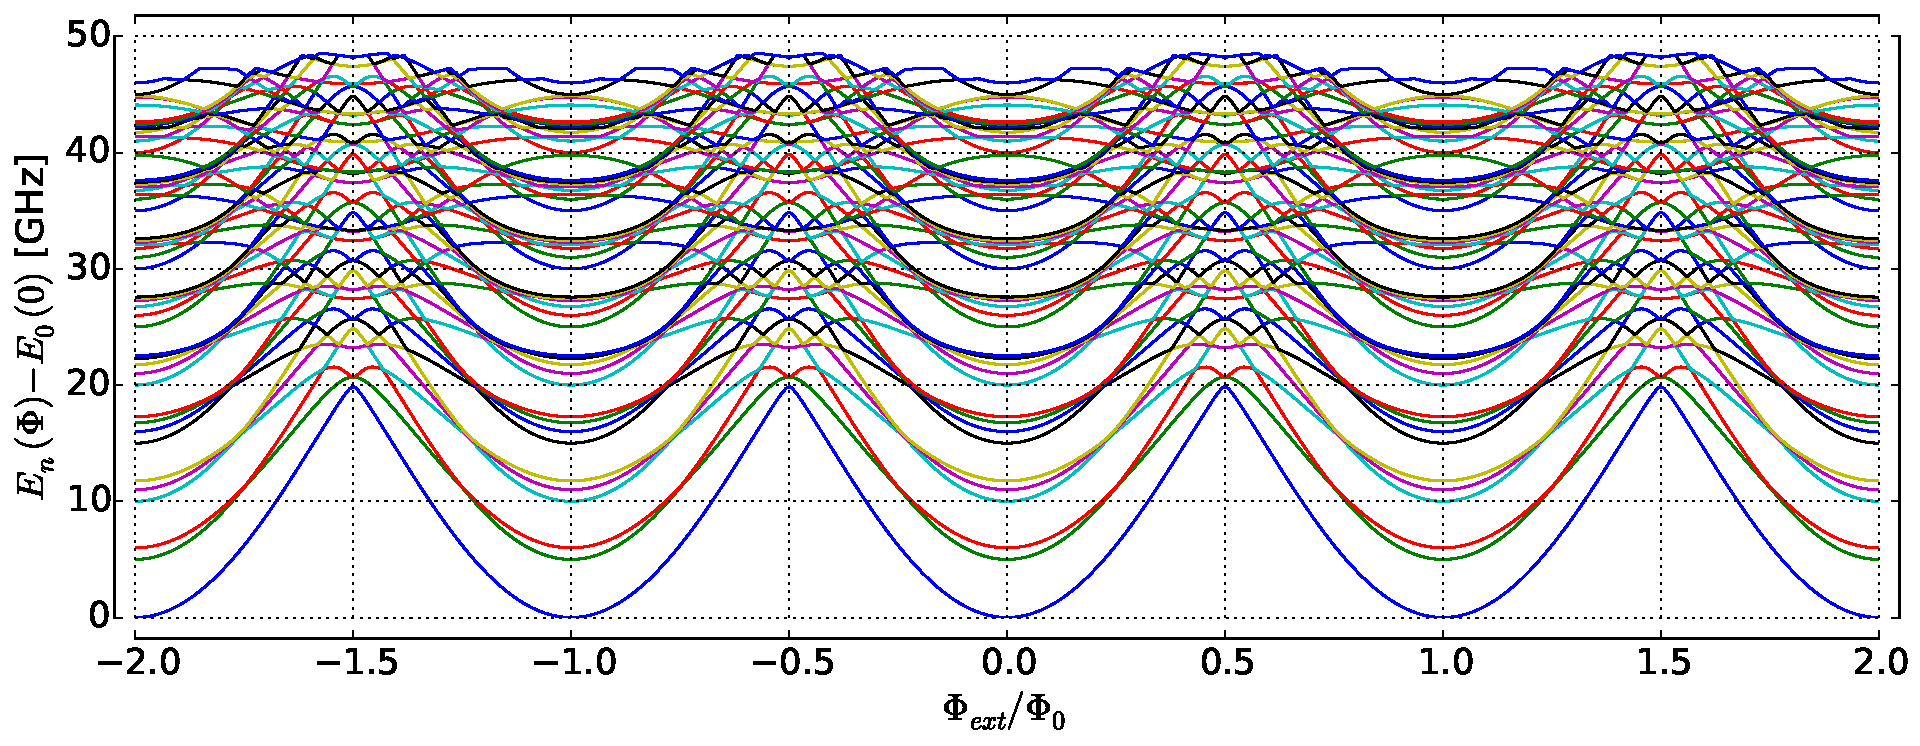
\includegraphics[width=0.9\textwidth]{levels}
\end{subfigure}

\begin{subfigure}[t]{\textwidth}
\centering
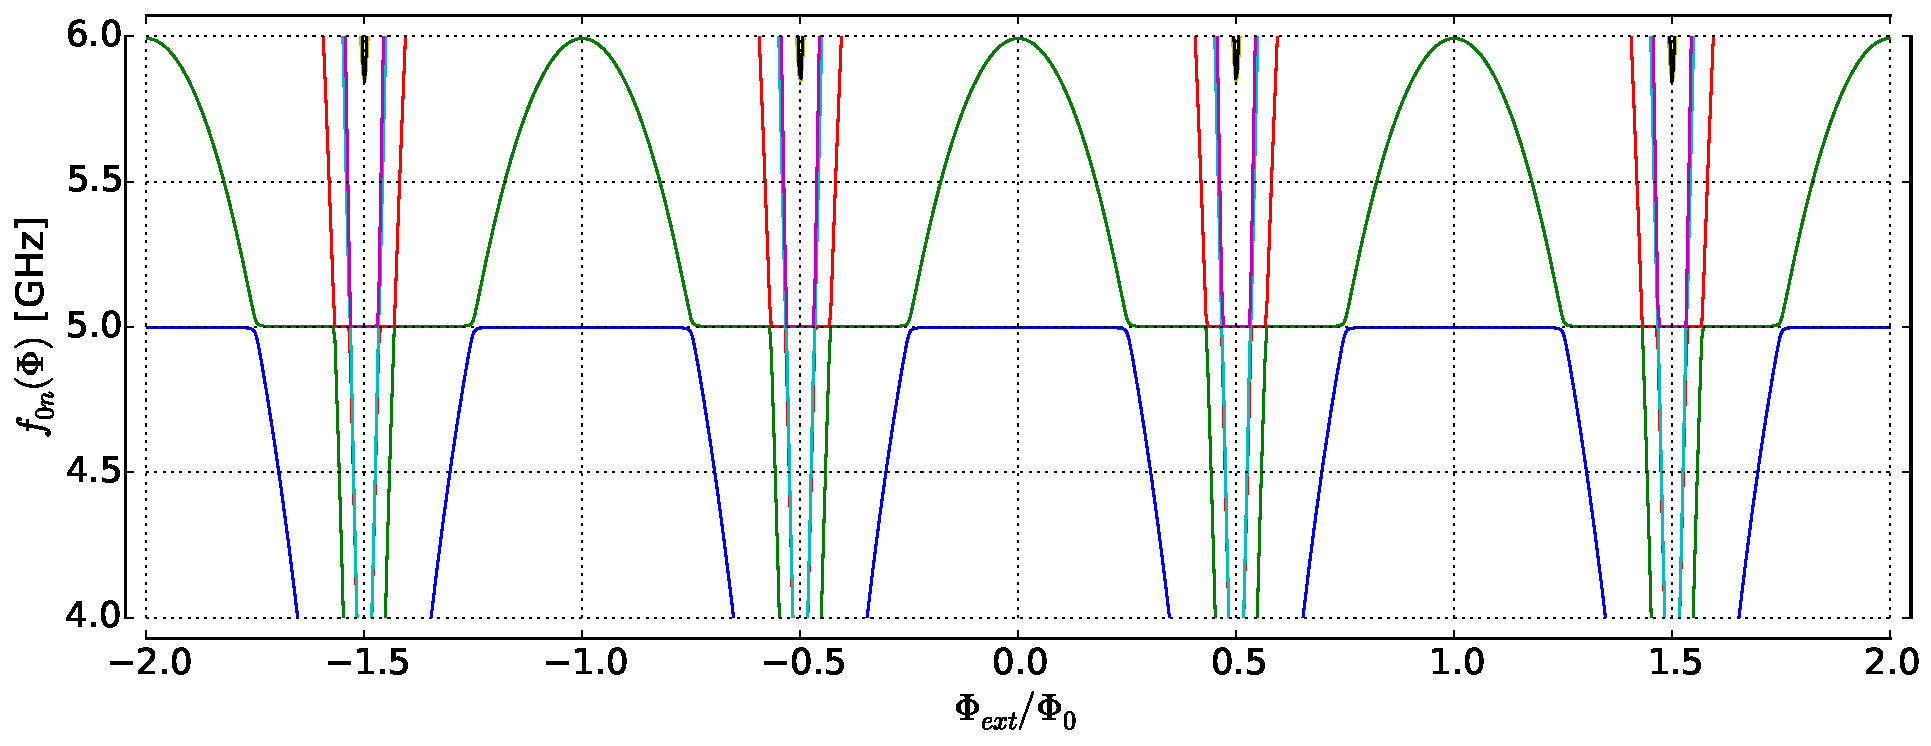
\includegraphics[width=0.9\textwidth]{freqs}
\end{subfigure}
\caption{Energy structure and transition frequencies (from the ground state) of the transmon-resonator system depending on $\Phi_{ext}$.}
\label{fig:levels}
\end{figure}


\begin{figure}[h]
\centering
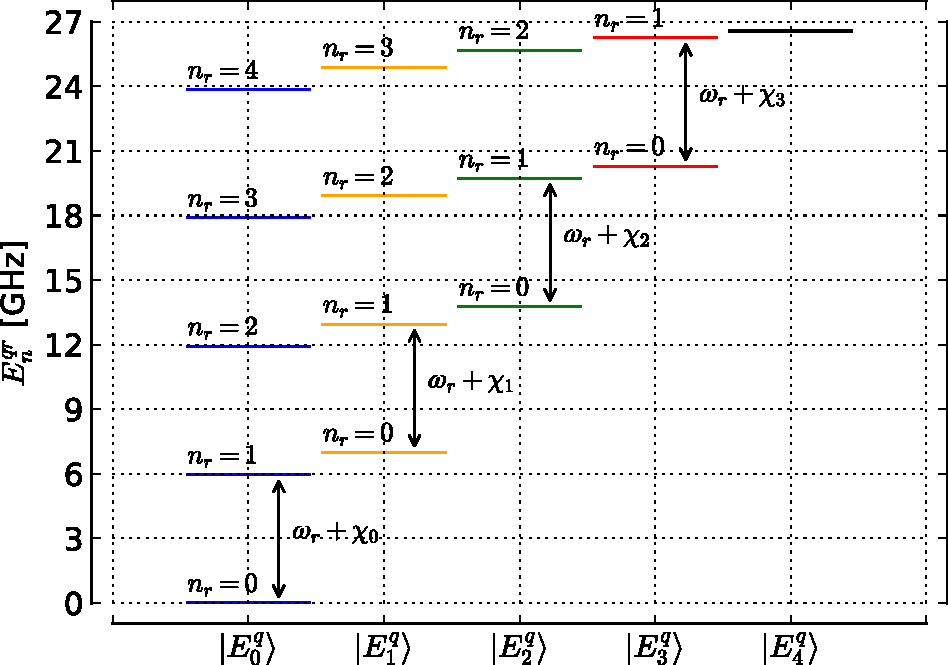
\includegraphics[height=0.25\textheight]{diagram_q>r}\ 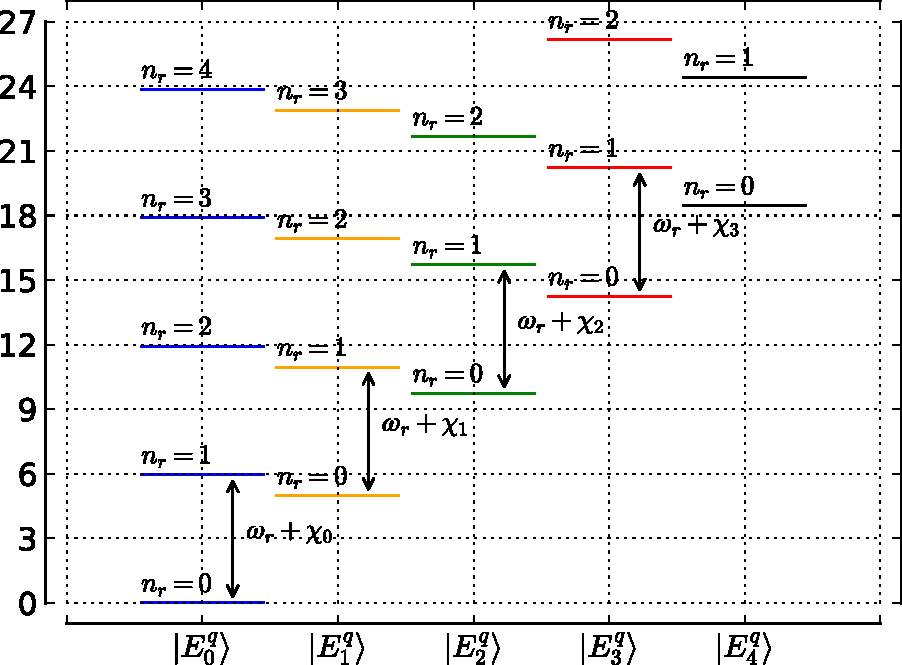
\includegraphics[height=0.25\textheight]{diagram_q<r}
\caption{Energy level diagrams for the transmon-resonator system in the sweet spot when the detuning $\Delta_\omega = \omega_r-\omega_{ge}$ is negative (right) or positive (left).}
\label{fig:diagram}
\end{figure}

\subsection{Energy spectrum of the transmon-resonator system}

Using QuTiP\cite{Johansson2011} it is easy to solve the truncated matrix eigenproblem with the Hamiltonian \eqref{eq:hamiltonian}. The results for the typical design values
$$
C_\kappa = 5 \text{ fF},\ C_g = 2 \text{ fF},\ C_q = 90 \text{ fF},\ C_r = 500 \text{ fF},\ L_r = 2 \text{ nH}, $$
$$E_{J, \Sigma} = (h \nu_q + E_C)^2/8 E_C\ \text{for\cite{Koch2007}}\ \nu_q = 6\ \text{GHz}
$$
can be observed in \autoref{fig:levels}.

In \autoref{fig:diagram} the energy structure of the compound system in the sweet-spot ($\Phi_{ext}=0$) is shown for two cases of positive and negative detuning. The dispersively shifted frequencies can be calculated from perturbation theory. For example, for the transition $\ket{0, g}\rightarrow \ket{1, g}$ the shift is defined to the second order as
\begin{align*}
\chi_0 &=  E_{1g}^{(1)} + E_{1g}^{(2)} - E_{0g}^{(1)} - E_{0g}^{(2)}\\
 &= \bra{1, g}\mathcal{\hat H}_i\ket{1,g} + \sum_{i, \alpha \neq 1, g} \frac{|\bra{g, 1}\mathcal{\hat H}_i\ket{i,\alpha} |^2}{E_{1g} - E_{i\alpha}}\\
 & - \bra{0, g}\mathcal{\hat H}_i\ket{0,g} - \sum_{i, \alpha \neq 0, g} \frac{|\bra{g, 0}\mathcal{\hat H}_i\ket{i,\alpha} |^2}{E_{1g} - E_{i\alpha}}.
\end{align*}
As long as $\mathcal{\hat H}_i$ mixes only adjacent resonator states the first order corrections vanish, and so do the summations over $i$: $\sum_{i, \alpha} \rightarrow \sum_{0,\alpha} + \sum_{2,\alpha} (\sum_{1,\alpha})$. These sums then can be further truncated:
\begin{equation}
E_{1g}^{(2)} - E_{0g}^{(2)} \approx \frac{|\bra{g,1}\mathcal{\hat H}_i\ket{0,e}|^2}{\omega_r - \omega_{ge}} + \frac{|\bra{g,1}\mathcal{\hat H}_i\ket{2,e}|^2}{\omega_r - 2\omega_r - \omega_{ge}} -
\frac{|\bra{g,0}\mathcal{\hat H}_i\ket{1,e}|^2}{-\omega_r - \omega_{ge}}\label{eq:chi0_truncsums}
\end{equation} 
due to the selection rule of $\hat n$: $\bra{E^q_n}\hat n \ket{E^q_{n+2k}} = 0,\ k \in \mathbb{Z}$ and the fast (exponential from numerics) decay of its matrix elements over distance between transmon energy eigenstates (see \autoref{sec:tr_eigen}). It can be easily proven that last two elements of \eqref{eq:chi0_truncsums} are equal up to the factor of $\sqrt{2}^2$ and final equation for $\chi_0$ follows
\begin{equation}
\chi_0 = g^2\sbrkt{\frac{n_{ge}^2}{\omega_r - \omega_{ge}}-\frac{n_{ge}^2}{\omega_r + \omega_{ge}}}.
\label{eq:chi0}
\end{equation}

\begin{figure}[h!]
\centering
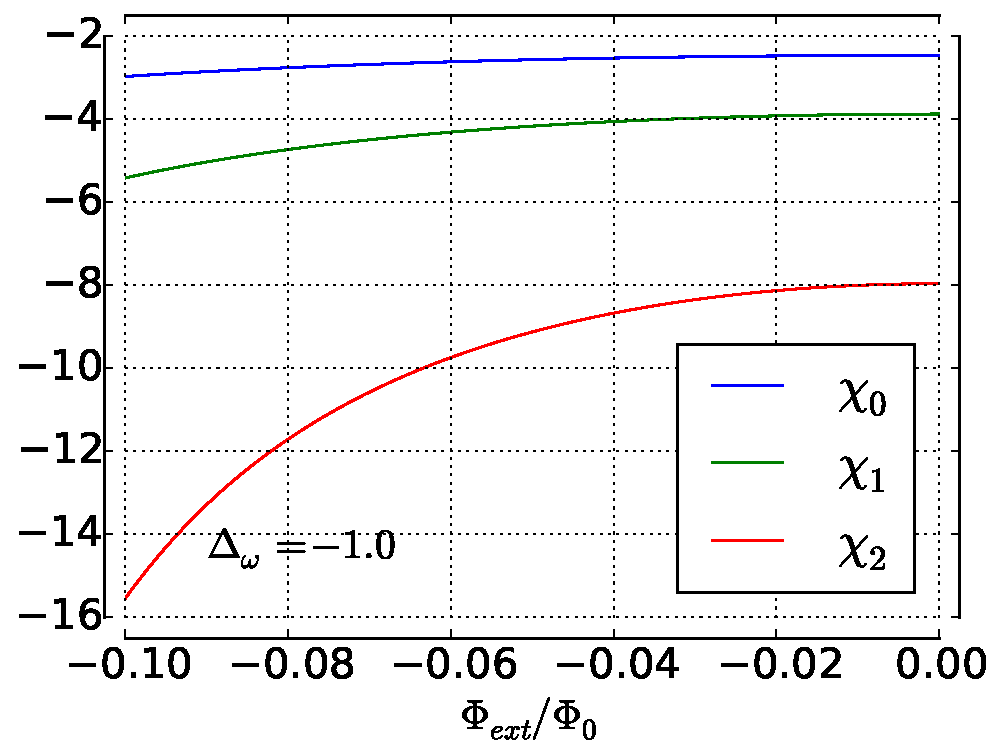
\includegraphics[height=0.25\textheight]{shifts-10.pdf}
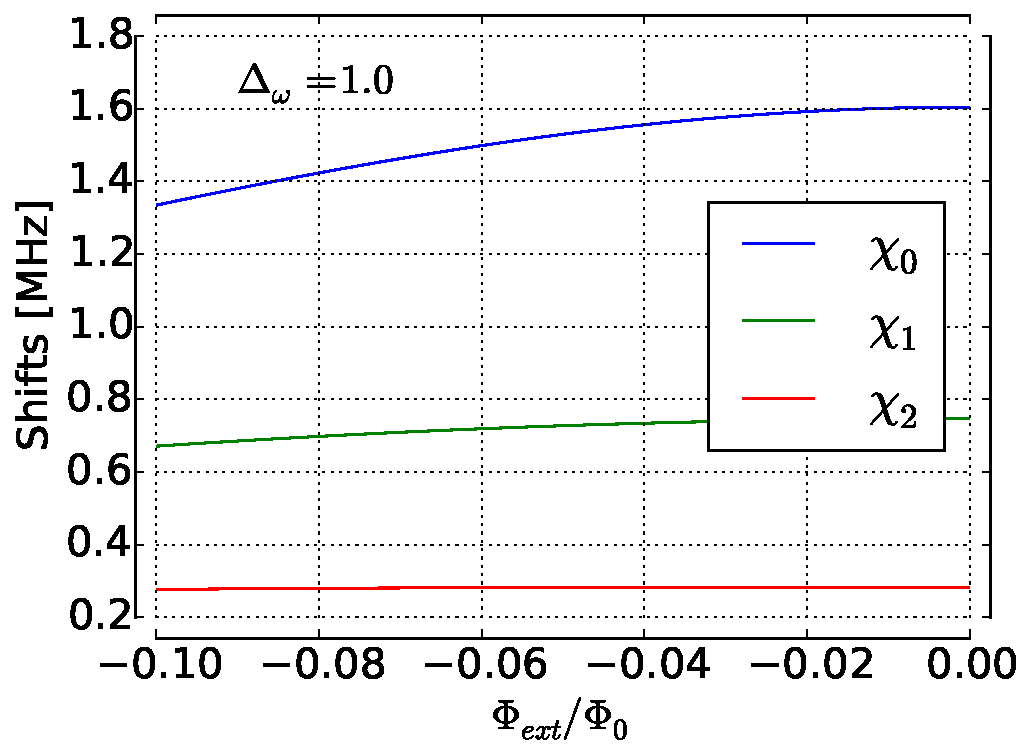
\includegraphics[height=0.25\textheight]{shifts10.pdf}
\caption{Dispersive shifts for the first three states of the transmon in dependence on the external flux. Solid lines are numerical solution and dashed lines are results from equations \eqref{eq:chi0}-\eqref{eq:chi2}.}
\label{fig:disp_shifts}
\end{figure}

Similarly, dispersive shifts for the other two transmon states are derived:
\begin{gather}
\chi_1 = g^2\sbrkt{\frac{n_{ef}^2}{\omega_r - \omega_{ef}} - \frac{n_{ef}^2}{\omega_r + \omega_{ef}} + \frac{n_{eg}^2}{\omega_r + \omega_{ge}}-\frac{n_{eg}^2}{\omega_r - \omega_{ge} }},\label{eq:chi1}
\\
\chi_2 = g^2\sbrkt{\frac{n_{fd}^2}{\omega_r - \omega_{fd}} -\frac{n_{fd}^2}{\omega_r + \omega_{fd}} + \frac{n_{fe}^2}{\omega_r + \omega_{ef}}- \frac{n_{fe}^2}{\omega_r -\omega_{ef}}},
\label{eq:chi2}
\end{gather}
where $g, e, f, d$ denote the first 4 energy eigenstates of the transmon, $n_{\alpha\beta} = \bra{\alpha} \hat n \ket{\beta}$ is the matrix element of $\hat n$ and $g = \left.|\frac{\mathcal{\hat H}_i}{i(\hat a^\dag  - \hat a)\otimes \hat n}|\right.$ is the coupling parameter which precedes the operator part in the interaction Hamiltonian. In \autoref{fig:disp_shifts} these formulas are compared to the numerical solution. As can be seen, the analytical solution is quite accurate at the detunings of about 1 GHz. Note that dispersive shift $\chi_1$ is always smaller than $\chi_0$ when the detuning is large enough meaning that the resonator frequency will move down from its initial position. There is also another regime which occurs when the resonator frequency is situated between transitions $ge$ and $ef$ and is called \textit{straddling regime} by Koch et al.\cite{Koch2007}. The dispersive regime breaks down there when the coupling is strong enough (i.e., 50 MHz) and the anharmonicity of the qubit is not very large (i.e., 200 MHz) compared to it, so the second order correction equations become inaccurate. In this regime, however, $\chi_1>\chi_0$, and the resonator moves up when the qubit is excited.


\section{Dynamics}\label{sec:dynamics}

\subsection{Driving of an isolated transmon}

To simulate the dynamics in the unitary case without taking into account the dissipative processes, it is enough to solve the Schrödinger equation with the Hamiltonian \eqref{eq:hamiltonian} summed with the driving part \eqref{eq:driving_q}. The final state after some time of the evolution $t$ will be described with a Dyson series or a $\hat T$-exponent:
\begin{equation}
\begin{aligned}
\ket{\psi (t)} &= \hat T \exp\left\{-\frac{i}{\hbar} \rbrkt{\mathcal{\hat H}_{tr}t + \int_0^t \mathcal{\hat H}_q^d(\tau) \diff\tau}\right\} \ket{\psi(0)}\\
&\equiv \hat U(t, 0) \ket{\psi(0)}\equiv \sum_k c_k(t) \ket{E^q_k},
\end{aligned}
\label{eq:dyson}
\end{equation} 
where $\ket{E_k^q}$ denotes the $k$'s eigenstate of the qubit Hamiltonian and $\hat U(t, 0)$ is the standard evolution operator. There is no exact analytical solution for $c_k(t)$ for the transmon qubit, so we will use some approximations, perturbation theory and numerical methods to get an insight into the dynamics of this quantum system.

\subsubsection{Approximate solution for two-level dynamics} \label{sec:tr_rwa}

Let's write down the matrix equation for the time-dependent Schrödinger's equation in the energy representation of the transmon:

\begin{equation*}
i\hbar \left(
\begin{matrix}
\dot c_g \\
\dot c_e\\
\dot c_f\\
\dot c_d\\
\vdots
\end{matrix}
\right) = 
\left[\left(
\begin{matrix}
E_g & 0 & 0 & 0 & \cdots\\
0 &E_e & 0 & 0 & \cdots\\
0 & 0 & E_f & 0 & \cdots\\
0 & 0 & 0 & E_d & \cdots\\
\vdots&\vdots&\vdots&\vdots& \ddots
\end{matrix}
\right)
+
f(t)
\left(
\begin{matrix}
0          & n_{ge} & 0         & n_{gd} & \cdots\\
n_{eg} & 0          & n_{ef} & 0         & \cdots\\
0          & n_{fe}  & 0         & n_{fd} & \cdots\\
n_{dg} & 0          & n_{df} & 0         & \cdots\\
\vdots&\vdots&\vdots&\vdots& \ddots
\end{matrix}
\right)\right]
\left(
\begin{matrix}
c_g\\
c_e\\
c_f\\
c_d\\
\vdots
\end{matrix}
\right).
\end{equation*}
Here we have used the properties of the $\hat n$ (see \autoref{sec:tr_eigen}) operator to simplify its matrix representation. Now we can write down the differential equations for three lowest levels:
\begin{equation}
\begin{cases}
i\hbar \dot c_g = E_g c_g + f(t) (n_{ge} c_e + n_{gd} c_d + \cdots),\\
i\hbar \dot c_e = E_e c_e + f(t) (n_{eg} c_g + n_{ef} c_f + \cdots),\\
i\hbar \dot c_f = E_f c_f + f(t) (n_{fe} c_e + n_{fd} c_d + \cdots).
\end{cases}
\label{eq:c_gef_ode}
\end{equation}
Then we use the following ansatz: $c_\alpha = c_\alpha' \exp( - i \frac{E_\alpha t}{\hbar})$, which transforms the Hamiltonian into the \textit{rotating frame} (or the \textit{interaction picture}). In this frame, the unperturbed Hamiltonian is equal to $\hat 0$, and the equations \eqref{eq:c_gef_ode} become (omitting apostrophes):

\begin{equation}
\begin{cases}
i\hbar \dot c_g =  f(t) (n_{ge} c_e e^{-i\omega_{ge}t}+ n_{gd} c_d  e^{-i\omega_{gd}t} + \cdots),\\
i\hbar \dot c_e =  f(t) (n_{eg} c_g e^{i\omega_{ge}t} + n_{ef} c_f e^{-i\omega_{ef}t}+ \cdots),\\
i\hbar \dot c_f =   f(t) (n_{fe} c_e e^{i\omega_{ef}t}+ n_{fd} c_d e^{-i\omega_{df}t} + \cdots).
\end{cases}
\label{eq:c_gef_ode_rf}
\end{equation}

Finally, assuming harmonic perturbation at $ge$ transition frequency, $f(t) = \hbar f \cos(\omega_{ge} t + \phi ) = \frac{\hbar f}{2}(e^{i\omega_{ge} t+i\phi} + e^{-i\omega_{ge} t-i\phi})$, and dropping all oscillating terms (\textit{rotating wave approximation, RWA}), we obtain the standard two-level dynamics for Rabi oscillations around the axis $-\phi$ degrees away from the $x$-axis of the Bloch sphere with angular frequency of $\Omega_R = f n_{ge}$:
\begin{equation}
\begin{cases}
i\hbar \dot c_g =  \frac{\hbar fe^{i\phi}}{2} n_{ge} c_e,\\
i\hbar \dot c_e =   \frac{\hbar fe^{-i\phi}}{2} n_{eg} c_g.
\end{cases} \Leftrightarrow\  i\partial_t \ket{\psi (t)} = \frac{\Omega_R}{2}[\cos(\phi)\hat \sigma_x - \sin(\phi)\hat \sigma_y]\ket{\psi(t)}.
\label{eq:rwa_ode}
\end{equation}

\begin{figure}
\centering
\includegraphics[width=.4\textwidth]{2d_rabi_example_bloch_pure}\quad
\includegraphics[width=.4\textwidth]{2d_rabi_example_bloch_pure_Y}
\caption{Visualization of the solution of \eqref{eq:rwa_ode} on the Bloch sphere for $\Omega_R=5$ MHz and two values of $\phi$: 0 (left) and $-\pi/2$ (right).}
\label{fig:bloch_rot}
\end{figure}

The exact solution for this equation may be obtained with use of the matrix exponent and the following properties of $\hat \sigma_{x,y}$: $\hat \sigma_x^2 = \mathbbm{\hat 1},\ \hat \sigma_x^3 = \hat\sigma_x$. However, since $\hat \sigma_x$ and $\hat \sigma_y$ are not commuting, it is a bit cumbersome to calculate the matrix exponent when $\phi$ is arbitrary, and it's easier just to switch the basis so that $\phi=0$. So below we solve the equation in this case:
\begin{equation}
\begin{aligned}
\ket{\psi(t)} &= \exp\{i\frac{\Omega_R}{2}\hat \sigma_x t\} \ket{\psi(0)}\\
& = \left[\mathbbm{\hat 1} \cos\left(\frac{\Omega_R}{2}  t\right) + i\hat \sigma_x \sin\left(\frac{\Omega_R}{2} t\right)\right]\ket{\psi(0)}. 
\end{aligned}
\end{equation}
With initial state $\ket{g}$, we can calculate the probability of being in the states $\ket{e}$ and $\ket{+} = \frac{1}{\sqrt{2}}(\ket{g}+\ket{e})$ to be  as follows:
\begin{equation}
\begin{aligned}
P(\ket{e})(t) &= |\braket{e}{\psi(t)}|^2 = \frac{1-\cos(\Omega_R t)}{2},\\
P(\ket{+})(t) &= |\braket{+}{\psi(t)}|^2 = \frac{1}{2}.
\end{aligned}
\label{eq:x_rotation}
\end{equation}
Clearly, this is by definition the rotation around the $x$-axis. The $y$ rotation may be derived in a similar way if the phase is chosen to be $-\pi/2$. 

In general, using these formulas, we can define $(\theta)^{x(y)}$-pulse as windowed sine wave with window of correct amplitude, duration and phase, so that the qubit is rotated $\theta$ radians around the corresponding axis (see \autoref{fig:bloch_rot}). For example, for a fixed-length pulse of $t_g$, the $(-\frac{\pi}{2})^{y}$-pulse amplitude $f_q$ should be $- \pi/2 t_g n_{ge}$ and pulse phase $\phi$ equal to $-\pi/2$. Conversely, for a fixed $\Omega_R$ (drive amplitude $f_q$) to perform the same rotation the pulse time $t_g$ should be chosen as $\pi/2\Omega_R$ for the excitation signal with the phase increased by $\pi$ (as $t_g\geq 0$).

\subsubsection{Time-dependent perturbation theory}

Perturbation theory allows semianalytical calculation of the transition rates	(Rabi oscillation frequencies) for single and multi-photon processes. Using the the Dyson series we can write down the expansion of the evolution operator $\hat U(t, t_0)$  and then use it to calculate the expansion of the transition rate $A_{fi} = \bra{f}\hat U(t, t_0)\ket{i}$ from some initial state $\ket{i}$ to the final state $\ket{f}$ under some driving operator $\hat V(t)$. Here is the result for the $\hat U(t, t_0)$ decomposition:\cite{faisal2013}
\begin{equation}
\begin{aligned}
\hat U(t, t_0) &= 1 + \sum_n \hat U^{(n)}(t, t_0),\\
\hat U^{(n)}(t, t_0) &= \left(-\frac{i}{\hbar}\right)^n\int\limits_{t_0}^t \diff t_1 \hat V_I(t_1)\int\limits_{t_0}^{t_1} \diff t_2 \hat V_I(t_2)\cdots\int\limits_{t_0}^{t_{n-1}} \diff t_n \hat V_I(t_n),
\end{aligned}
\end{equation}
where $\hat V_I(t) = \exp(i\mathcal{\hat H}_{tr}(t-t_0)/\hbar) \hat V(t) \exp(-i\mathcal{\hat H}_{tr}(t-t_0)/\hbar)$ is the driving operator in the interaction picture (same as in the rotating frame). For example, let's reproduce the previous result and calculate the Rabi frequency for the single-photon transition.  The transition rate $A^{(1)}_{eg}(t) = \bra{e}\hat U^{(1)}(t, t_0)\ket{g}$ when $\hat V(t) = \hbar f \hat n \cos(\omega t)$ is calculated as follows :
\begin{equation}
A^{(1)}_{eg}(t) = - i \frac{f n_{eg}}{2} \int\limits_{t_0}^t e^{i\omega_{ge} t_1} (e^{i\omega t_1}+e^{-i\omega t_1})\diff t_1.
\end{equation}
In the limit of ${t-t_0\gg1/\omega}$ and $\omega - \omega_{ge}\ll1$ this can be rewritten as
\[
A^{(1)}_{eg}(t) \sim - i \frac{f n_{eg}}{2} t.
\]
Consequently, $P(\ket{e}) = |A_{eg}|^2 = (f n_{eg}/2)^2t^2$, and this is exactly the first term of the expansion of the first formula in \eqref{eq:x_rotation} thus giving us the same Rabi frequency of $f n_{eg}$. 

Multi-photon transition rates are harder to calculate since they require summations over different intermediate states $\ket{j}$ between the initial and the final state. Nevertheless, below we will calculate the Rabi frequency of the two-photon $gf/2$ transition, so that $\omega \approx \omega_{gf}/2$. The first order correction vanishes for this transition, and thus we need to calculate the second order correction only. Following Faisal\cite{faisal2013}, we obtain:
\[
A^{(2)}_{fg}(t) \sim  i (f/2)^2 \sum_j \frac{n_{fj}n_{jg}}{\omega_{gj}-\omega_{gf}/2} t \approx  i (f/2)^2 \frac{n_{fe}n_{eg}}{\omega_{ge}-\omega_{gf}/2} t.
\]
Analogously to the previous case, this gives us the two-photon Rabi frequency: 
\begin{equation}
\Omega_{R, gf}^{2p} = \frac{f^2  n_{fe}n_{eg}}{|\alpha|} ,
\label{eq:rabi_2p}
\end{equation}
where $\alpha$ is the anharmonicity of the transmon. Note that it is proportional to the squared drive strength -- a standard result for a 2-photon process. This formula will be tested numerically in the section below.
 
\begin{figure}[h!]
\centering
\includegraphics[width=0.32\textwidth]{tr_10.0MHz_dr}
\includegraphics[width=0.32\textwidth]{tr_100.0MHz_dr}
\includegraphics[width=0.32\textwidth]{tr_200.0MHz_dr}
\caption{Dynamics of the isolated driven transmon qubit with different drive strengths $f_q/2\pi$ = 0.01-0.2 GHz, where $f_q$ is an effective amplitude of the drive \eqref{eq:driving_q} $f_q (t) = \hbar  f_q \cos(\omega_{ge} t)$. It can be seen that significant distortions and leakage to higher levels occur when amplitude becomes comparable to the transmon's anharmonicity.}
\label{fig:driven_tr}
\end{figure}

\begin{figure}[h!]
\centering
\includegraphics[height=0.185\textheight]{tr_xyz10}\includegraphics[height=0.185\textheight]{tr_xyz20}\includegraphics[height=0.185\textheight]{tr_xyz50}
\caption{Numerical solution for the two-level behaviour of the transmon in the computational basis for different drive strengths. Note the phase error due to the leakage to the higher levels which is growing with the driving strength and is noticeable even when the drive strength is small compared to the anharmonicity.}
\label{fig:xyz_tr}
\end{figure}

\subsubsection{Numerical solution for two-level dynamics}

The simulation of the transmon dynamics can be performed as a standard numerical linear ODE solution which is also possible within QuTiP framework using the \textit{mesolve} routine. Below the results for the following model will be presented:
\[
\mathcal{\hat H} = \mathcal{\hat H}_{tr}  +\mathcal{\hat H}_q^d(t),\ f_q^d(t) =\hbar f_q \cos(\omega_{ge}t),\ \omega_{ge}/2\pi = 6\ \text{GHz},\ \alpha/2\pi = - 200\ \text{MHz}.
\]
We can solve the time-dependent Schrödinger equation with this Hamiltonian with $\ket{g}$ as the initial state to obtain system state $\ket{\psi(t)}$ as each time point we need, and then calculate the projections of these states onto the eigenstates to find decomposition coefficients $c_{g}..c_{d}$. Alternatively, it is possible to  find the expectation values for the quasi-two-level operators
\[
\hat \sigma_x = \ket{g}\bra{e}+\ket{e}\bra{g},\ \hat\sigma_y = i\ket{g}\bra{e} - i\ket{e}\bra{g},\ \hat\sigma_z  = \ket{e}\bra{e}-\ket{g}\bra{g}
\]
for each state $\ket{\psi(t)}$ which allow us to find its phase in the \textit{computational basis}. However, when higher levels are involved in the dynamics, these expectation values loose their meaning and should be used with discretion.

The result of such simulations can be observed in \autoref{fig:driven_tr} and \autoref{fig:xyz_tr}. As one can see, when the driving amplitude becomes comparable to the anharmonicity of the transmon, significant leakage to higher states occurs which in the computational basis manifests itself as a phase error. This error is significant even when the driving strength is relatively small, so special techniques such as Derivative Removal by Adiabatic Gate\cite{Motzoi2009,Chow2010} (DRAG) or Half Derivative\cite{Lucero2010} (HD) method were suggested to cope with it.

DRAG procedure can correct any continuous pulse rotating the qubit around some axis (i.e., $(\pi)^x$) by adding two simultaneous pulses around two other axes. If the  $(\pi)^x$-pulse has the windowing function $F_x(t)$, the pulses around $y$-axis and $z$-axis (which is usually just a DC-pulse, i.e., pulse with no carrier, providing dynamic detuning of the qubit during this operation) should be constructed as follows:
\[
F_y = -\frac{\dot F_x}{\alpha},\ \omega-\omega_{ge}(t) = \frac{(\lambda^2-4)F_x^2}{4\alpha}
\]
However, it is possible to alleviate the necessity of $z$-pulses by putting $F_y=-\frac{1}{2}\frac{\dot F_x}{\alpha}$. This change significantly reduces the complexity of the original DRAG operation while maintaining approximately the same performance, as numerical simulations has shown\cite{Lucero2010}. The resulting operation is named the Half Derivative method after the factor of 1/2 before $\dot F_x$, and not because it is somehow connected to fractional calculus.

\begin{figure}
\centering
\includegraphics[width=0.32\textwidth]{tr_2p_1MHz_dr} \includegraphics[width=0.32\textwidth]{tr_2p_5MHz_dr} \includegraphics[width=0.32\textwidth]{tr_2p_10MHz_dr}
\caption{Simulated two-photon $gf/2$ Rabi oscillations. The Rabi frequency is closer to the theoretically predicted one in \eqref{eq:rabi_2p} when the drive is weak and deviates more and more when the drive strength is increased. Higher-frequency oscillations are present, too, and also grow with the drive amplitude.}
\label{fig:2p_sim}
\end{figure}

\subsubsection{Numerical solution for two-photon dynamics}

Similarly to the single-photon two-level process simulated above, we can simulate the two-photon transition $gf/2$. To test the equation \eqref{eq:rabi_2p}, we put $f_q$ which is the amplitude of the two-photon driving $f_q \cos(\omega_{fg}/2+t)$ to be as follows:
\[
f_q = \sqrt{\frac{\Omega_{R,gf}^{2p} |\alpha|}{n_{ge}n_{ef}}},
\]
where $\Omega_{R,gf}^{2p}$ is the two-photon Rabi frequency which we want to observe. The results of the numerical simulation performed with this method are presented in \autoref{fig:2p_sim}. For $\Omega_{R,gf}^{2p}/2\pi =$ 1 MHz (5 MHz, 10 MHz), we observe the two-photon Rabi frequency of 1.03 MHz (5.2 MHz, 11 MHz) which is a good match considering the perturbative nature of the the equation \eqref{eq:rabi_2p}. 

\begin{figure}
\includegraphics[width=.5\textwidth]{tr_decay}\hspace{-7.5cm}\textbf{(a)}\hspace{6.5cm}
\includegraphics[width=.5\textwidth]{tr_str_dr_decay}\hspace{-7.5cm}\textbf{(b)}\hspace{6.5cm}
\caption{Behaviour of the equation \eqref{eq:tr_dissip_dyn}, represented as populations of the eigenstates depending on time. \textbf{(a)} Relaxation of the first excited state without any driving. The population reaches $1/e$ in $1/\gamma$ ns, as expected. \textbf{(b)} Excitation of the ground state into the steady state which is an incoherent mixture of the first three states. Driving is resonant with the $ge$ transition of the transmon.}
\end{figure}

\subsection{Relaxation dynamics (driven and undriven)}

The relaxation process for the transmon is simulated using a Lindbladian master equation with a following dissipative operator:
\begin{equation}
\hat c = \sum_{j\geq 0}^\infty \frac{n_{j\,j+1} }{n_{01}}\ket{j}\bra{j+1}
\end{equation}
which is from the definition a lowering operator. It becomes the annihilation operator of the standard harmonic oscillator in the limit of very large $E_J/E_C$, so it is a good operator to model the relaxation channel. For a deeper review on this, see L.S. Bishop's PhD thesis.\cite{Bishop2010}

The dynamics of the dissipative transmon then will be governed by the following equation:
\begin{equation}
\frac{\partial}{\partial t} \hat{\rho}_q = \frac{i}{\hbar}[\hat{\rho}_q, \hat{\mathcal{H}}_q+\hat{\mathcal{H}}_q^d(t)] + \gamma \mathcal{D}[\hat c]\hat\rho_q,
\label{eq:tr_dissip_dyn}
\end{equation}
where $ \mathcal{D}[\hat{\mathcal{O}}]\hat\rho_q = \hat{\mathcal{O}} \hat\rho_q \hat{\mathcal{O}}^\dag - \frac{1}{2}\{\hat{\mathcal{O}}^\dag \hat{\mathcal{O}}, \hat\rho_q \}$ and $\gamma$ is the relaxation rate. Pure dephasing may also be added in a similar way.

Below the dynamics of the undriven relaxation and excitation with strong driving are presented as examples of the solution of \eqref{eq:tr_dissip_dyn}.

\subsection{Linewidth dependence on drive power} \label{subsec:linewidth}

\subsubsection{Two-level model}

Knowing the way to model the relaxation of the qubit, it is possible to compare the relaxation rate with the linewidth of the qubit on the population graph. The way is to simulate the evolution until the steady state is reached for all driving frequencies around the resonance, calculate populations of the excited state for each reached steady state and then measure the width at the half-maximum of the resulting peak. However, for two-level dynamics the linewidth $\delta \omega$ depends on the driving power as the Rabi oscillations are induced between the levels. So for correct determination of the linewidth it's necessary to measure the linewidth at low driving amplitudes.

Before demonstrating the numerical results for the transmon qubit, a brief analytical solution for the problem in the case of a two-level system will be shown. The master equation for this problem is as follows (within the RWA):
\[
\frac{\partial}{\partial t} \hat{\rho}_{tls} = \frac{i}{\hbar}[\hat{\rho}_{tls}, \frac{\hbar (\overbrace{\omega_{tls}-\omega_d}^{\Delta\omega})}{2} \hat{\sigma}_z+\frac{\hbar \Omega_R}{2} \hat{\sigma}_x] + \gamma \mathcal{D}[\hat \sigma^-]\hat\rho_{tls}.
\]
Knowing that $\text{Tr}[\hat\rho_{tls}]=1$ and that $\hat\rho_{tls}=\hat\rho_{tls}^\dag$ we can write down three ODEs from this master equation:
\[
\begin{gathered}
\frac{d}{d t} {ρ_{11}}{\left (t \right )} = - γ {ρ_{11}}{\left (t \right )} + i \left(\frac{Ω_{R}}{2} {ρ_{12}}{\left (t \right )} - \frac{Ω_{R}}{2} {ρ_{21}}{\left (t \right )}\right), \\
\frac{d}{d t} {ρ_{12}}{\left (t \right )} = - \frac{γ}{2} {ρ_{12}}{\left (t \right )} + i \left( \frac{Ω_{R}}{2} {ρ_{11}}{\left (t \right )} - \frac{Ω_{R}}{2} \left(1- {ρ_{11}}{\left (t \right )} \right) - \Delta ω {ρ_{12}}{\left (t \right )}\right),\\
{ρ_{21}}{\left (t \right )} = {ρ_{12}}^\dag{\left (t \right )}.
\end{gathered}
\]

It is practical for our case to solve these equations for the \textit{steady state}, when $\frac{\partial}{\partial t} \hat{\rho}_{tls} = 0$. The matrix elements then are
\[
ρ_{11} = \frac{Ω_{R}^{2}}{2 Ω_{R}^{2} + γ^{2} + 4 \Delta ω^{2}},\quad
ρ_{12} = - \frac{Ω_{R} \left(i γ + 2 \Delta ω\right)}{2 Ω_{R}^{2} + γ^{2} + 4 \Delta ω^{2}},\quad
ρ_{21} = \frac{Ω_{R} \left(i γ - 2 \Delta ω\right)}{2 Ω_{R}^{2} + γ^{2} + 4 \Delta ω^{2}}.
\]

From here it is easy to find the analytical linewidth at half maximum of the $\rho_{11}(\omega_d)$:
\[
\delta\omega = \sqrt{2\Omega_R^2+\gamma^2}.
\]

When the $\Omega_R \rightarrow 0,\ \delta\omega\rightarrow\gamma$, and thus it is possible to extract $T_1$ in case of absence of pure dephasing, or at least to put a lower bound on it if pure dephasing is present. It is important to notice that in the experiment the measured frequency is expressed in Hz though $\delta\omega$ is in rad/s. Therefore, the experimental linewidth should be, firstly, measured at very low powers and, secondly, multiplied by $2\pi$ to obtain $\gamma$. In the presence of pure dephasing the formula for $\delta\omega$ becomes a bit more complicated, but also can be straightforwardly calculated with use of Computer Algebra Systems:
\[
\delta\omega_{\text{with dephasing}} = \sqrt{2Ω_{R}^{2} (1+2 γ_{ϕ}/\gamma) + (\gamma +2\gamma_\phi)^2} \xrightarrow[\Omega_R\rightarrow 0]{} γ + 2γ_{ϕ}.
\]

Interestingly enough, if there's no relaxation and $\gamma = 0$, the formula shows divergence of the linewidth. This happens because the solution of the master equation in this case yields $\rho_{11} = 1/2$ in the steady state, independent of the driving detuning and driving strength, and thus the linewidth can not at all be defined.


\begin{figure}
\centering
\includegraphics[width=\textwidth]{transmon_transtitions_narroww_gamma5e-3}

\includegraphics[width=0.7\textwidth]{linewidth_prop_ss}
\caption{Linewidth analysis in dependence on the driving power $f_q$ for $\gamma = 5$ rad/$\mu$s. As can be seen, with the increasing drive amplitude the spectral line becomes wider. In contrast, its width levels off when the amplitude is decreased, and reaches asymptotically the value of $\frac{\gamma}{2\pi}$. The factor $2\pi$ appears as long as the linewidth found in the experiment usually is in Hz, but the equality that holds is that $\gamma = \delta\omega$, and $\delta\omega = 2\pi\delta\nu$.}
\label{fig:transmon_lw}
\end{figure}  
\subsubsection{Transmon case}

For the transmon, the two-level dynamics between its ground and first excited state is equivalent; however, there's no simple analytical solution for the dynamics between many levels. To see the behaviour is the same in this case we have to resort to numerical modelling (see \autoref{fig:transmon_lw}). As can be seen, the linewidth $\delta\omega$ grows with the increased power, and, in contrast, saturates at low powers, reaching the value of $\gamma$. The growth is exponential meaning that the linewidth is indeed proportional to the Rabi frequency similarly as what the two-level model predicts. This is expected as long as the lowering operator $\hat c$ in the computational basis is exactly equal to $\hat \sigma^-$, and, as long as the system stays inside this basis, the dynamics is completely equivalent to the one predicted by the two-level master equation. 

In contrast, when the drive strength is increased beyond the anarmonicity of the transmon, we observe clear deviations from the two-level behaviour. The numerical simulations and experimental data show that additional multi-photon transitions begin to arise, and, besides the spectral line $ge$ we have seen in \autoref{fig:transmon_lw}, we will observe several other lines appearing at higher drive amplitudes. The resulting spectrum is presented in  

\begin{figure}
\centering
\includegraphics[width=\textwidth]{transmon_transtitions}
\caption{Different single- and multi-photon transitions in a transmon predicted by the full numerical model with relaxation. The parameters are the same as in the previous simulations.}
\end{figure}